\documentclass[11pt]{article}
\usepackage[utf8]{inputenc}
\usepackage[margin=1in]{geometry}
\usepackage{amsmath,amssymb,amsthm}
\usepackage{microtype}
\usepackage{hyperref}
\usepackage{booktabs}
\usepackage{enumitem}
\usepackage{tikz}
\usetikzlibrary{positioning}
\usepackage{xcolor}
\usepackage{float}

\definecolor{fieldblue}{HTML}{D6EAF8}
\definecolor{matrixgreen}{HTML}{D5F5E3}
\definecolor{metayellow}{HTML}{FEF9E7}
\definecolor{challgray}{HTML}{E8E8E8}

% Theorem environments
\newtheorem{theorem}{Theorem}[section]
\newtheorem{lemma}[theorem]{Lemma}
\newtheorem{proposition}[theorem]{Proposition}
\newtheorem{corollary}[theorem]{Corollary}
\newtheorem{definition}[theorem]{Definition}
\newtheorem{remark}[theorem]{Remark}

% Convenience macros
\newcommand{\Fp}{\mathbb{F}_p}
\newcommand{\Fpq}{\mathbb{F}_{p^2}}
\newcommand{\End}{\mathrm{End}}
\newcommand{\Z}{\mathbb{Z}}

\title{Signature Compression for SQIsign via Weil Pairing Recovery}
\author{
  Dustin Ray\thanks{Anchorage Digital, Security Engineering. \texttt{dustin@anchorage.com}} \and
  Paulo S.\,L.\,M.\ Barreto\thanks{University of Washington Tacoma. \texttt{pbarreto@uw.edu}}
}
\date{\today}

\begin{document}
\maketitle

\begin{abstract}
The SQIsign v2.0 specification~\cite{sqisign-spec-r2} transmits the full
$2 \times 2$ change-of-basis matrix $\mathbf{M}_{\mathrm{chl}}$ in every
signature. Dropping one entry and recovering it from the Weil pairing is a
technique introduced by Basso, Maino and Pope for FESTA~\cite{festa} and
applied to SQIsignHD by Dartois et al.~\cite{sqisignhd}. The v2.0
specification neither implements it nor states the recovery formula for
its two-dimensional response. We state and prove that formula from the
specification's own definitions. The Weil pairing of the transmitted basis
of the challenge curve, raised to the determinant, times the Weil pairing
of the auxiliary basis, is a primitive fourth root of unity. Hence the determinant is known modulo
$2^{e_{\mathrm{rsp}} - n_{\mathrm{bt}} + 1}$, one bit short of the width at
which the matrix is carried, and that bit is the only free one. We give an
adaptive pivot for the signatures whose leading entry is even. With a
one-bit hint, basis-hint recomputation and metadata packing, the level~I
signature becomes 129 bytes, 19 below the 148 of the specification. The
construction is checked on the 300 NIST known-answer vectors at levels I,
III and V. We explain why the reduced
Tate pairing on the transmitted basis is useless here: its arguments are
$2^{F - N}$-th multiples of full-order points, so its values have order
at most $2^{2N - F}$. On the deterministic bases scaled to order $2^m$ a single
Tate ladder recovers the determinant once $2m - F$ reaches the precision,
on all 300 vectors. At level~I that is one ladder of 187 steps against
two of 128. The round-3 specification of
September 2026 also transmits the full matrix; the same recovery at its
parameters gives 176, 269 and 353 bytes against 200, 306 and 406, measured
on its 300 known-answer vectors.
\end{abstract}

\paragraph{Keywords.} SQIsign, isogeny-based cryptography, signature compression,
Weil pairing, post-quantum cryptography.

\tableofcontents
\newpage

%% ============================================================
\section{Introduction}
\label{sec:intro}
%% ============================================================

SQIsign~\cite{sqisign-original} is an isogeny-based post-quantum digital
signature scheme whose combined public-key-plus-signature size (213 bytes
at NIST Level~I) is roughly $7\times$ smaller than FN-DSA and $17\times$
smaller than ML-DSA.
% source: sqisign-spec-r2 Section 1.1 (7x Falcon, 16 to 17x ML-DSA) and
% Table 1 (65 + 148 = 213). SQIsign advanced to Round~2 of the NIST Post-Quantum
Cryptography Additional Signatures standardization
process~\cite{nist-pqc-sig} in 2025, with an updated v2.0
specification~\cite{sqisign-spec-r2} based on the SQIsign2D-West
construction of Basso et al.~\cite{sqisign2d-west}. The v2.0 scheme
replaces the KLPT-based response of v1.0 with interpolation data
transmitted as a $2 \times 2$ change-of-basis matrix
$\mathbf{M}_{\mathrm{chl}}$ over $\mathbb{Z}/2^N\mathbb{Z}$, yielding
148-byte signatures at Level~I. A round-3 specification with new
parameters followed in September 2026~\cite{sqisign-spec-r3}; this paper
treats SQIsign v2.0 and v2.0.1 (round 2), and round 3 in
Section~\ref{sec:round3}.
% source: sqisign-spec-r2 Table 1 (148 bytes); sqisign-spec-r3 title page (date).

Compact signatures are especially valuable in bandwidth-constrained
settings: TLS certificate chains, embedded attestation protocols, and
blockchain transaction throughput all improve with smaller signatures.
Every byte removed from the wire format compounds across millions of
handshakes or blocks.

\paragraph{The determinant-recovery idea is known.}
Recovering a dropped matrix coefficient from the Weil pairing determinant
relation was introduced in the context of FESTA by Basso, Maino, and
Pope~\cite{festa}. They observed that ``given three of the four
coefficients representing the scaled points, it is possible to retrieve
the fourth one via the compatibility of the Weil pairing with
isogenies.'' Nakagawa and Onuki applied the same principle in
QFESTA~\cite{qfesta}. Dartois et al.\ deployed it in
SQIsignHD~\cite{sqisignhd}, where the response matrix is compressed to
three of four scalars with recovery via the determinant equation
$a_1 b_2 - b_1 a_2 \equiv kq \pmod{\ell^f}$. The SQIsignHD paper
further notes the invertibility pivot: ``If $a_1$ is invertible, we can
recover $b_2$ from the other scalars \ldots\ and we can recover $a_2$
otherwise.'' The earlier SIDH key-compression literature also uses
pairing-based scalar recovery~\cite{costello-compression, zanon2018,
naehrig-renes}.

\paragraph{The specification gap.}
Despite this lineage, the SQIsign v2.0 specification~\cite{sqisign-spec-r2}
transmits all four entries of $\mathbf{M}_{\mathrm{chl}}$ (Table~3 of the
spec). Pairings appear only in Algorithm~2.5 (\textsc{ChangeOfBasis}) to
\emph{compute} the full matrix during signing; no algorithm, footnote, or
wire format in the specification implements the drop-and-recover
compression for the dim\nobreakdash-2 response structure. The v2.0.1
update~\cite{sqisign-spec-v201} does not change this. Nakagawa and
Onuki~\cite{sqisign2dpush} confirm that SQIsign2DPush signatures ``can be
compressed similarly to SQIsign-v2.0,'' corroborating that the v2.0
baseline does not apply scalar recovery.

\paragraph{Lineage.}
We first wrote the technique down for the reference implementation's
maintainers on 8 July 2026, as issue~19 of its repository, ``Technical
notes on signature compression techniques''~\cite{issue19}. Luca De~Feo
replied for the team the same day that ``we may introduce some compression
in round 3, depending on performance''. On 7 October 2026 he added that
``we will give a closer look at compression for the next round''. The
issue cites a comment in \texttt{biextension.c} of the round-2 reference
at tag \texttt{nist-v2} (commit \texttt{91e9e46})~\cite{the-sqisign-v2}.
It reads: ``If we work with full order points, it would be faster to use
the Tate pairings rather than the Weil pairings; this is not implemented
yet.''
% source: github.com/SQISign/the-sqisign/issues/19 (read 2026-10-22);
% the-sqisign nist-v2, src/ec/ref/lvlx/biextension.c lines 311-314.

\paragraph{Contributions.}
We fill this gap with the following concrete results, each situated
against the prior work it builds on.

\begin{enumerate}[label=(\arabic*)]

\item \textbf{The recovery formula for the v2.0 response matrix, with a
proof from the specification} (\S\ref{sec:formula}). Let $(A, B)$ be the
deterministic basis of $E_{\mathrm{chl}}[2^N]$ and $(C, D)$ that of
$E_{\mathrm{aux}}[2^{N - r_{\mathrm{rsp}}}]$ as the verifier scales them,
$\omega = e_{2^N}(A, B)$ and $\eta = e_{2^{N - r_{\mathrm{rsp}}}}(C, D)$.
Theorem~\ref{thm:main} states that $\omega^{\det \mathbf{M}} \eta$ is a
primitive fourth root of unity for every honestly generated signature, so
\[
  \det(\mathbf{M}) \;\equiv\; \log_{\omega}\bigl(\eta^{-1}\bigr)
  \pmod{2^{g}}, \qquad g = e_{\mathrm{rsp}} - n_{\mathrm{bt}}.
\]
The proof uses only bilinearity, alternation, compatibility with isogenies
and the signer's Kani square. The response degree $q$ cancels against the
auxiliary degree $2^{e'} - q$. The formula is confirmed on all 300 NIST
KAT vectors.

\item \textbf{Precision: one free bit} (\S\ref{sec:formula}). The matrix
is carried modulo $2^N$ with $N = g + 2$, the 2 being the extra torsion
of the specification's $(2,2)$-isogeny chain. The theorem fixes the
parity of the quotient $(\det \mathbf{M} - \log_\omega \eta^{-1}) / 2^g$,
so a discrete logarithm taken at order $2^N$ determines $\det \mathbf{M}$
modulo $2^{N - 1}$ and leaves a single free bit, bit $N - 1$.

\item \textbf{Adaptive pivot} (\S\ref{sec:pivot}). The determinant has
2-adic valuation $r_{\mathrm{rsp}}$. When it is odd and $M_{00}$ is even,
$M_{01}$ is odd and the decompressor drops $M_{10}$ instead of $M_{11}$,
with the path read off the parity of $M_{00}$. We report how often each
case occurs on the KAT vectors.

\item \textbf{Compression from 148 to 129 bytes} (\S\ref{sec:compression}):
the Weil recovery (148 to 133), the one-bit hint (133 to 132), basis-hint
recomputation (132 to 130) and metadata packing (130 to 129), with the bit
layouts.

\item \textbf{Pairing selection and negative results}
(\S\ref{sec:negative}). The reduced Tate pairing on the transmitted basis
is degenerate because its arguments are $2^{F - N}$-th multiples of
full-order points, not because of the final exponentiation. We derive the
order of its values as a function of the ladder length and measure it on
every order from $2^N$ to $2^F$. On the full-order points a single Tate
ladder recovers the determinant, because the reduced Tate pairing is
alternating on these curves; we report where that becomes cheaper than
two Weil ladders. We also document why the hint cannot be dropped by
signer retry and why 128 bytes needs a signer-side canonical form.

\item \textbf{Implementation, costs, and round 3} (\S\ref{sec:impl},
\S\ref{sec:round3}). A pure Rust \texttt{no\_std} verifier validates all
three formats on the 300 KAT vectors; we break the cost of compressed
verification into its components. On the round-3 parameters the same
recovery gives 176, 269 and 353 bytes, measured on the 300 round-3 KAT
vectors.

\end{enumerate}

\subsection{Related work}

The isogeny key-compression literature begins with Costello et
al.~\cite{costello-compression}, who introduced point compression for SIDH
public keys. Zanon et al.~\cite{zanon2018} (journal
version~\cite{zanon2019}) accelerated SIDH key compression via Tate
pairings and reverse basis decomposition. Naehrig and
Renes~\cite{naehrig-renes} developed dual-isogeny-based compression for
SIDH. Pereira and Barreto~\cite{pereira-barreto} eliminated the pairing
entirely via Pohlig-Hellman on the elliptic curve group; we discuss the
applicability of this technique to SQIsign decompression
in~\S\ref{sec:conclusion}.

For SQIsign optimization, Aardal et al.~\cite{aardal2024} achieved
record verification times (8.55 Mcycles on Raptor Lake, 5.6 Mcycles for
uncompressed signatures) using assembly-level optimization and
multi-core parallelism.
% source: \cite{aardal2024}, abstract. Corte-Real Santos et al.~\cite{apressqi}
introduced extension-field signing for faster verification. Kim et
al.~\cite{kim2026} reduced quaternion precision budgets by 74 to 75\%.
% source: \cite{kim2026}, abstract.
De~Feo et al.~\cite{sqisign-arm} provided the first vectorized (NEON)
SQIsign implementation.

Robert~\cite{robert-pairings} and Pope et al.~\cite{pope-pairings}
developed faster cubical/biextension pairing algorithms with direct
applicability to SQIsign; our Weil pairing computation follows their
approach.

A complete security proof for SQIsign was given by Aardal et
al.~\cite{sqisign-security}.

\subsection{Notation}
\label{sec:notation}

The specification writes $f$ for the 2-adic valuation of $p + 1$
(Table~3 and Section~4.2.1 of~\cite{sqisign-spec-r2}). We write $F$ for
it, to keep $f$ free, and $v_2(n)$ for the 2-adic valuation of an integer
$n$, the largest $k$ with $2^k \mid n$. All other quantities are the
specification's. Per level: $\lambda = 128, 192, 256$;
$c = 5, 65, 27$; $F = 248, 376, 500$; $e_{\mathrm{rsp}} = 126, 192, 253$;
$e_{\mathrm{chl}} = 122, 184, 247$.
% source: sqisign-spec-r2 Chapter 5 (p, c, lambda) and Appendix B
% (f, e_rsp, e_chl); the same values are the crate's params/level*.rs
% constants at v0.4.31 (F_CHR, E_RSP).

\begin{center}
\begin{tabular}{l p{10.5cm}}
\toprule
\textbf{Symbol} & \textbf{Meaning} \\
\midrule
$\lambda$ & Security parameter, 128, 192 or 256. \\
$p$ & The prime, $p = c \cdot 2^F - 1$ with $c$ odd; Chapter~5 of~\cite{sqisign-spec-r2}. \\
$F$ & $v_2(p + 1)$, the exponent of the accessible 2-torsion ($f$ in the specification); 248, 376, 500. \\
$e_{\mathrm{rsp}}$ & $\lceil \log_2 \sqrt{p} \rceil$, the response bound (Section~4.2.1); 126, 192, 253. \\
$e_{\mathrm{chl}}$ & $F - e_{\mathrm{rsp}}$, the bit length of the challenge; 122, 184, 247. \\
$n_{\mathrm{bt}}$, $r_{\mathrm{rsp}}$ & Backtracking steps and $v_2(\deg \varphi_{\mathrm{rsp}})$, carried in the signature (Section~4.4.3). \\
$e'$ & $e_{\mathrm{rsp}} - r_{\mathrm{rsp}} - n_{\mathrm{bt}}$, the length of the $(2,2)$-chain (Algorithm~4.2, line~20). \\
$N$ & $e' + r_{\mathrm{rsp}} + 2 = e_{\mathrm{rsp}} - n_{\mathrm{bt}} + 2$, the bit width of a matrix entry (Algorithm~4.9, line~5). \\
$g$ & $N - 2 = e_{\mathrm{rsp}} - n_{\mathrm{bt}}$, the precision of the recovery. \\
$E_0$ & The curve $y^2 = x^3 + x$ with its fixed basis $B_0 = (P_0, Q_0)$ of $E_0[2^F]$. \\
$E_{\mathrm{pk}}, E_{\mathrm{com}}, E_{\mathrm{chl}}, E_{\mathrm{aux}}$ & Public-key, commitment, challenge and auxiliary curves. \\
$(A, B)$ & The deterministic basis of $E_{\mathrm{chl}}[2^F]$ scaled to order $2^N$ (Algorithm~4.9, lines 12 and 13). \\
$(C, D)$ & The deterministic basis of $E_{\mathrm{aux}}[2^F]$ scaled to order $2^{e' + 2}$ (lines 10 and 11). \\
$\mathbf{M}$ & $\mathbf{M}_{\mathrm{chl}}$, entries $M_{00}, M_{01}, M_{10}, M_{11}$ in wire order, in $[0, 2^N)$. \\
$e_n(\cdot, \cdot)$ & The Weil pairing of order $n$; $\mu_n$ the $n$-th roots of unity in $\mathbb{F}_{p^2}^*$. \\
$\omega$, $\eta$ & $e_{2^N}(A, B)$ and $e_{2^{e' + 2}}(C, D)$. \\
\bottomrule
\end{tabular}
\end{center}



%% ============================================================
\section{Preliminaries}
\label{sec:prelim}
%% ============================================================

\subsection{Supersingular elliptic curves and isogenies}

We recall the definitions needed to fix notation. For a full treatment of
elliptic curves we refer to Silverman~\cite{silverman}, and for a survey
of isogeny-based cryptography to De~Feo~\cite{defeo-survey}.

Let $p$ be a prime with $p \equiv 3 \pmod{4}$. A supersingular elliptic
curve over $\mathbb{F}_{p^2}$ is an elliptic curve whose
$\mathbb{F}_{p^2}$-rational endomorphism ring is an order in a quaternion
algebra rather than an imaginary quadratic field. SQIsign works
exclusively with supersingular curves in Montgomery form
$E_{A}: By^2 = x^3 + Ax^2 + x$ over $\mathbb{F}_{p^2}$, where the
$j$-invariant is determined by $A$ alone. The base curve is
$E_0: y^2 = x^3 + x$ (i.e., $A = 0$, $B = 1$) with known endomorphism
ring $\mathcal{O}_0 \cong \mathrm{End}(E_0)$.

An isogeny $\varphi: E \to E'$ is a non-constant morphism of elliptic
curves preserving the identity. Its degree $\deg(\varphi)$ equals the size
of its kernel $\ker(\varphi)$. Every isogeny of degree $d$ has a dual
isogeny $\hat{\varphi}: E' \to E$ satisfying
$\hat{\varphi} \circ \varphi = [d]_E$ and
$\varphi \circ \hat{\varphi} = [d]_{E'}$, where $[d]$ denotes the
multiplication-by-$d$ map. An isogeny is cyclic if its kernel is a cyclic
group, in which case it is determined up to post-composition by an
automorphism by a single kernel generator $K \in E[d]$.

SQIsign uses $x$-only arithmetic on Montgomery curves throughout: points
are represented by their $x$-coordinate (or projective
$(X : Z)$ pairs), and the $y$-coordinate is avoided except where pairings
require it. This follows the approach detailed in
Costello and Hisil~\cite{costello-hisil} and adopted in the SQIsign
specification~\cite{sqisign-spec-r2}.

For an integer $N$ coprime to $p$, the $N$-torsion subgroup
$E[N] = \{P \in E(\overline{\mathbb{F}_p}) : [N]P = \mathcal{O}\}$
is isomorphic to $(\mathbb{Z}/N\mathbb{Z})^2$. A basis $(P, Q)$ of
$E[N]$ satisfies $E[N] = \langle P \rangle \oplus \langle Q \rangle$,
and the Weil pairing $e_N(P, Q)$ is a primitive $N$-th root of unity.
The SQIsign specification fixes a deterministic basis of $E[2^F]$ on
each curve, generated with a one-byte hint by Algorithm~2.1
(\textsc{TorsionBasisToHint}) and rebuilt from the hint by Algorithm~2.2
(\textsc{TorsionBasisFromHint}). The choice of this basis is central to
the compression formula of~\S\ref{sec:formula}.

\subsection{The SQIsign v2.0 signature scheme}

We summarize the protocol at the level of detail needed to understand the
compression; the full specification is in~\cite{sqisign-spec-r2} and the
underlying construction in~\cite{sqisign2d-west}. A security proof
appears in~\cite{sqisign-security}.

SQIsign is a sigma protocol turned into a signature via the Fiat-Shamir
transform~\cite{fiat-shamir}. The prover demonstrates knowledge of
$\mathrm{End}(E_{\mathrm{pk}})$, which is computationally equivalent to
knowing an isogeny path from the public base curve $E_0$ to the public key
curve $E_{\mathrm{pk}}$.

\paragraph{Key generation.}
The signer samples a random isogeny
$\tau: E_0 \to E_{\mathrm{pk}}$ of smooth degree $D_{\tau}$. The public
key is the Montgomery coefficient $A_{\mathrm{pk}}$ of
$E_{\mathrm{pk}}$ (64 bytes at Level~I); the secret key is the ideal
$I_{\tau}$ in $\mathrm{End}(E_0)$ corresponding to $\tau$ under the
Deuring correspondence~\cite{sqisign-deuring}.

\paragraph{Signing.}
Given a message $\mathsf{msg}$, the signer:
\begin{enumerate}[label=\arabic*., nosep]
\item \emph{Commits:} samples a random isogeny
  $\psi: E_0 \to E_{\mathrm{com}}$ and publishes $E_{\mathrm{com}}$.
\item \emph{Receives a challenge:} the verifier (or, via Fiat-Shamir,
  the hash function) produces a challenge isogeny
  $\varphi_{\mathrm{chl}}: E_{\mathrm{pk}} \to E_{\mathrm{chall}}$
  of degree $2^{e_{\mathrm{chl}}}$ determined by the hash
  $\mathsf{chl} = \mathsf{HASH}(A_{\mathrm{pk}}, A_{\mathrm{com}},
  \mathsf{msg})$.
\item \emph{Responds:} using knowledge of $\mathrm{End}(E_{\mathrm{pk}})$,
  the signer finds an isogeny $\sigma: E_{\mathrm{com}} \to E_{\mathrm{chall}}$
  of degree $q \approx \sqrt{p}$.
\end{enumerate}
The critical change from v1.0 is step~3. The original SQIsign required
$\sigma$ to have smooth degree, found via the KLPT
algorithm~\cite{sqisign-original, sqisign-deuring}. SQIsign
v2.0~\cite{sqisign2d-west} requires only that $q$ be small (not
necessarily smooth) and represents $\sigma$ by its action on torsion
points. A dimension-2 isogeny embedding via Kani's lemma~\cite{kani}
makes that representation efficiently evaluable by the verifier.

Concretely, the signer constructs an auxiliary isogeny
$\varphi_{\mathrm{aux}}: E_{\mathrm{com}} \to E_{\mathrm{aux}}$ such
that $q + \deg(\varphi_{\mathrm{aux}}) = 2^{e_{\mathrm{rsp}}}$, and
encodes $\sigma$ as a $2 \times 2$ change-of-basis matrix
$\mathbf{M}_{\mathrm{chl}}$ over $\mathbb{Z}/2^N\mathbb{Z}$. This matrix
expresses, in the deterministic basis of $E_{\mathrm{chall}}$, the images
under the response of a basis of $E_{\mathrm{com}}[2^N]$. That basis of
$E_{\mathrm{com}}$ is chosen so that the auxiliary isogeny maps it onto
the deterministic basis of $E_{\mathrm{aux}}$ (Algorithm~4.8 of the
specification; \S\ref{sec:formula} makes this precise). The signature is
\[
  (\mathsf{chl},\, A_{\mathrm{aux}},\, \mathbf{M}_{\mathrm{chl}},\,
  n_{\mathrm{bt}},\, r_{\mathrm{rsp}},\, \mathsf{hint}_{\mathrm{aux}},\,
  \mathsf{hint}_{\mathrm{chall}}).
\]

\paragraph{Verification.}
The verifier reconstructs $E_{\mathrm{chall}}$ from the public key and
the challenge scalar, and regenerates the deterministic torsion bases on
$E_{\mathrm{chall}}$ and $E_{\mathrm{aux}}$ from the transmitted hints.
It applies $\mathbf{M}_{\mathrm{chl}}$ to obtain the torsion-point images
of $\sigma$ and constructs from them the Kani $(2^a, 2^a)$-isogeny
$\Phi: E_{\mathrm{chall}} \times E_{\mathrm{aux}} \to
E_{\mathrm{com}} \times E'_{\mathrm{aux}}$. It evaluates
$\Phi$ to recover $E_{\mathrm{com}}$, and checks that
$\mathsf{chl} = \mathsf{HASH}(A_{\mathrm{pk}}, A_{\mathrm{com}},
\mathsf{msg})$.

Compression modifies only the first stage of this flow: recovering the
full $\mathbf{M}_{\mathrm{chl}}$ from a reduced representation before
proceeding with the standard verification. Everything from the Kani
embedding onward is unchanged.

\subsection{Signature wire format}
\label{sec:wireformat}

Table~3 of the specification~\cite{sqisign-spec-r2} defines the standard
signature as the tuple
\[
  (\mathsf{chl},\, A_{\mathrm{aux}},\, \mathbf{M}_{\mathrm{chl}},\,
  n_{\mathrm{bt}},\, r_{\mathrm{rsp}},\, \mathsf{hint}_{\mathrm{aux}},\,
  \mathsf{hint}_{\mathrm{chall}}).
\]
At NIST Level~I ($\lambda = 128$, $F = 248$, $e_{\mathrm{rsp}} = 126$)
the byte-level breakdown is as follows. A matrix entry occupies
$\lceil (e_{\mathrm{rsp}} + 2) / 8 \rceil$ bytes, 16, 25 and 32 at the
three levels, which is what the reference implementation and the sizes
of Table~1 of the specification use.\footnote{Appendix~B of
\cite{sqisign-spec-r2} prints the entry size as
$\lfloor (e_{\mathrm{rsp}} + 7)/8 \rfloor$, which gives 24 at level~III
and a 220-byte signature, against the 224 of its Table~1. The
implementation's $\lceil (e_{\mathrm{rsp}} + 2)/8 \rceil = 25$ is the
one consistent with the table.}
% source: sqisign-spec-r2 Appendix B (SIGNATURE_BYTES, Table 1) and the
% crate's matrix_entry_bytes() at v0.4.31.

\begin{center}
\begin{tabular}{l l r p{6.5cm}}
\toprule
\textbf{Field} & \textbf{Type} & \textbf{Bytes} & \textbf{Purpose} \\
\midrule
$A_{\mathrm{aux}}$ & $\mathbb{F}_{p^2}$ element & 64
  & Montgomery coefficient of $E_{\mathrm{aux}}$. \\
$\mathsf{chl}$ & integer & 16
  & Challenge scalar; verifier recomputes $\varphi_{\mathrm{chl}}$ from
    this and $E_{\mathrm{pk}}$. \\
$M_{00},\, M_{01}$ & scalars mod $2^N$ & $2 \times 16$
  & First row of $\mathbf{M}_{\mathrm{chl}}$: coefficients expressing
    $\sigma(P)$ in the canonical basis of $E_{\mathrm{aux}}$. \\
$M_{10},\, M_{11}$ & scalars mod $2^N$ & $2 \times 16$
  & Second row of $\mathbf{M}_{\mathrm{chl}}$: coefficients for
    $\sigma(Q)$. \\
$n_{\mathrm{bt}}$ & integer & 1
  & Number of backtracking steps in the response isogeny computation. \\
$r_{\mathrm{rsp}}$ & integer & 1
  & $v_2(\deg \varphi_{\mathrm{rsp}})$, the length of the even part of the
    response. \\
$\mathsf{hint}_{\mathrm{aux}}$ & byte & 1
  & Disambiguates the deterministic basis of $E_{\mathrm{aux}}[2^F]$. \\
$\mathsf{hint}_{\mathrm{chall}}$ & byte & 1
  & Disambiguates the deterministic basis of $E_{\mathrm{chl}}[2^F]$. \\
\midrule
& & \textbf{148} & \\
\bottomrule
\end{tabular}
\end{center}

The matrix $\mathbf{M}_{\mathrm{chl}}$ occupies 64 of the 148 bytes
(43\%). In FESTA~\cite{festa}, QFESTA~\cite{qfesta} and
SQIsignHD~\cite{sqisignhd} the determinant of the transmitted matrix is
tied to the degree of the represented isogeny. The relation has the form
$\det \mathbf{M} \equiv k \cdot q$, with $k$ fixed by the pairings of the
bases. In SQIsign v2.0 the auxiliary isogeny takes the place of $q$ and
the relation becomes the one of Theorem~\ref{thm:main}. In the standard
format the specification transmits all four entries and uses no such
relation.
% source: 64 = 4 x 16 bytes, Section 2.3 table; 64/148 = 0.432.

At Levels~III and~V the field sizes scale with $\lambda$, producing
224-byte and 292-byte signatures respectively. The matrix fraction
remains roughly 43\% at all levels.

\subsection{The Weil pairing}

For background on pairings over elliptic curves we refer to
Silverman~\cite{silverman}; for the specific computational methods used
in SQIsign we refer to Robert~\cite{robert-pairings} and Pope et
al.~\cite{pope-pairings}.

Let $N$ be a positive integer coprime to $\mathrm{char}(\mathbb{F}_q)$.
The Weil pairing $e_N: E[N] \times E[N] \to \mu_N$ maps pairs of
$N$-torsion points to $N$-th roots of unity in $\mathbb{F}_{q^k}^*$,
where $k$ is the embedding degree. Three of its properties matter for
the recovery formula:

\begin{enumerate}[label=(\roman*), nosep]
\item \emph{Bilinearity:}
  $e_N(P_1 + P_2,\, Q) = e_N(P_1, Q)\, e_N(P_2, Q)$, and
  symmetrically in the second argument.
\item \emph{Antisymmetry:}
  $e_N(P, Q) = e_N(Q, P)^{-1}$.
\item \emph{Non-degeneracy:} if $(P, Q)$ is a basis of $E[N]$, then
  $e_N(P, Q)$ is a primitive $N$-th root of unity.
\end{enumerate}

Property~(ii) distinguishes the Weil pairing from the Tate pairing,
which satisfies $\hat{t}_N(P, Q) = \hat{t}_N(Q, P)$ (symmetry, not
antisymmetry) after the final exponentiation. The relationship between
the two pairings, and the role of the torsion order in determining
whether the Tate pairing can substitute for the Weil pairing in
determinant recovery, is analyzed in~\S\ref{sec:negative}.

The SQIsign specification computes pairings via a biextension cubical
ladder on Montgomery curves (Section~8.3 of~\cite{sqisign-spec-r2}).
Pope et al.~\cite{pope-pairings}, building on
Robert~\cite{robert-pairings}, showed that this approach yields a
$>$40\% speedup over Miller's algorithm for the pairing orders used in
SQIsign.
% source: \cite{pope-pairings}, abstract.
The specification uses the Tate pairing for change-of-basis
computations during signing (Section~2.2.5.2
of~\cite{sqisign-spec-r2}). It notes that ``one may also use the Weil
pairing to compute the change of basis, although at an increase in
cost.''

%% ============================================================
\section{The decompression formula}
\label{sec:formula}
%% ============================================================

\subsection{What the verifier holds}
\label{sec:setting}

Fix a public key $(E_{\mathrm{pk}}, \mathsf{hint}_{\mathrm{pk}})$ and a
signature $\sigma = (E_{\mathrm{aux}}, n_{\mathrm{bt}}, r_{\mathrm{rsp}},
\mathbf{M}, \mathsf{chl}, \mathsf{hint}_{\mathrm{aux}},
\mathsf{hint}_{\mathrm{chl}})$ accepted by Algorithm~4.9 of the
specification~\cite{sqisign-spec-r2}. Write
$e' = e_{\mathrm{rsp}} - r_{\mathrm{rsp}} - n_{\mathrm{bt}}$,
$N = e' + r_{\mathrm{rsp}} + 2$ and $g = N - 2$ as in
\S\ref{sec:notation}. The verifier computes the following objects.
\begin{enumerate}[label=(\roman*), nosep]
\item $E_{\mathrm{chl}}$ from $E_{\mathrm{pk}}$ and $\mathsf{chl}$
  (line~9), the deterministic basis $(P^{\mathrm{det}}_{\mathrm{chl}},
  Q^{\mathrm{det}}_{\mathrm{chl}})$ of $E_{\mathrm{chl}}[2^F]$ from
  $\mathsf{hint}_{\mathrm{chl}}$ (line~12), and
  $A = [2^{F - N}] P^{\mathrm{det}}_{\mathrm{chl}}$,
  $B = [2^{F - N}] Q^{\mathrm{det}}_{\mathrm{chl}}$ (line~13), a basis of
  $E_{\mathrm{chl}}[2^N]$.
\item The deterministic basis of $E_{\mathrm{aux}}[2^F]$ from
  $\mathsf{hint}_{\mathrm{aux}}$ (line~10), and
  $C = [2^{F - e' - 2}] P^{\mathrm{det}}_{\mathrm{aux}}$,
  $D = [2^{F - e' - 2}] Q^{\mathrm{det}}_{\mathrm{aux}}$ (line~11), a
  basis of $E_{\mathrm{aux}}[2^{e' + 2}]$.
\item $P = [M_{00}] A + [M_{10}] B$ and $Q = [M_{01}] A + [M_{11}] B$
  (line~14).
\end{enumerate}
The entries are transmitted in the order $M_{00}, M_{01}, M_{10}, M_{11}$
(Section~4.6 of the specification), and (iii) is how the reference
implementation applies them: the first column acts on the first basis
point. Section~1.4 of the specification writes the same product with
$(A, B)$ as a column vector, which transposes the index names. Nothing
below depends on the choice except the names of the pivot entries in
\S\ref{sec:pivot}, which follow the implementation.
% source: sqisign-spec-r2 Algorithm 4.9 lines 9-14 and Section 4.6; the
% reference's matrix application (R = [a]P + [b]Q with a = M[0][0], b =
% M[1][0]) and the crate's matrix_scalar_application_even_basis at v0.4.31.

Define
\[
  \omega = e_{2^N}(A, B) \in \mu_{2^N}, \qquad
  \eta = e_{2^{e' + 2}}(C, D) \in \mu_{2^{e' + 2}} \subseteq \mu_{2^N}.
\]
Both are primitive roots of unity of their orders, since each is the Weil
pairing of a basis, and $\mu_{2^N} = \langle \omega \rangle$.

\subsection{What the matrix records}
\label{sec:records}

The signer (Algorithm~4.2 of the specification) produces a response
isogeny $\varphi_{\mathrm{rsp}} = \varphi^{\mathrm{even}}_{\mathrm{rsp}}
\circ \varphi^{\mathrm{odd}}_{\mathrm{rsp}} : E_{\mathrm{com}} \to
E_{\mathrm{chl}}$ with $\deg \varphi^{\mathrm{odd}}_{\mathrm{rsp}} = q$
odd (line~18) and $\deg \varphi^{\mathrm{even}}_{\mathrm{rsp}} =
2^{r_{\mathrm{rsp}}}$ (line~17 and Algorithm~4.6), and an auxiliary
isogeny $\varphi_{\mathrm{aux}} : E_{\mathrm{com}} \to E_{\mathrm{aux}}$
of degree $2^{e'} - q$ (line~23). Let $R_0 = [2^{F - N}]
\varphi_{\mathrm{com}}(P_0)$ and $S_0 = [2^{F - N}]
\varphi_{\mathrm{com}}(Q_0)$; since $\deg \varphi_{\mathrm{com}}$ is odd,
$(R_0, S_0)$ is a basis of $E_{\mathrm{com}}[2^N]$. The points the
signer carries into Algorithm~4.8 are (page~42 of the specification,
after Algorithms 4.6 and 4.7)
\[
  (P_{\mathrm{chl}}, Q_{\mathrm{chl}}) =
    (\varphi_{\mathrm{rsp}}(R_0), \varphi_{\mathrm{rsp}}(S_0)),
  \qquad
  (P_{\mathrm{aux}}, Q_{\mathrm{aux}}) =
    (\varphi_{\mathrm{aux}}(R_0), \varphi_{\mathrm{aux}}(S_0)),
\]
all of order $2^N$. Algorithm~4.8 computes a matrix $\mathbf{M}_1$ that
expresses the deterministic basis of $E_{\mathrm{aux}}[2^N]$ in
$(P_{\mathrm{aux}}, Q_{\mathrm{aux}})$ (line~5), applies $\mathbf{M}_1$ to
$(P_{\mathrm{chl}}, Q_{\mathrm{chl}})$ (line~6), and expresses the result
in the deterministic basis of $E_{\mathrm{chl}}[2^N]$. That matrix is
$\mathbf{M}_{\mathrm{chl}}$ (line~7). Put $(R, S) = \mathbf{M}_1 \cdot
(R_0, S_0)$, again a basis of $E_{\mathrm{com}}[2^N]$ because
$\mathbf{M}_1$ is invertible. Isogenies are linear, so:

\begin{lemma}
\label{lem:records}
For a signature produced by Algorithm~4.2 there is a basis $(R, S)$ of
$E_{\mathrm{com}}[2^N]$ such that
\[
  P = \varphi_{\mathrm{rsp}}(R), \quad
  Q = \varphi_{\mathrm{rsp}}(S), \quad
  C = \varphi_{\mathrm{aux}}([2^{r_{\mathrm{rsp}}}] R), \quad
  D = \varphi_{\mathrm{aux}}([2^{r_{\mathrm{rsp}}}] S).
\]
\end{lemma}

\begin{proof}
With $(R, S)$ as above, the deterministic basis of
$E_{\mathrm{aux}}[2^N]$ is $(\varphi_{\mathrm{aux}}(R),
\varphi_{\mathrm{aux}}(S))$ by line~5 of Algorithm~4.8. Since
$2^{F - e' - 2} = 2^{r_{\mathrm{rsp}}} \cdot 2^{F - N}$, the pair $(C, D)$
is its $[2^{r_{\mathrm{rsp}}}]$-multiple by (ii) of \S\ref{sec:setting}. Lines 6 and 7 of
Algorithm~4.8 say that $\mathbf{M}_{\mathrm{chl}}$ applied to the
deterministic basis of $E_{\mathrm{chl}}[2^N]$ is
$(\varphi_{\mathrm{rsp}}(R), \varphi_{\mathrm{rsp}}(S))$, which is (iii).
\end{proof}

\subsection{Pairing facts}

We use the following properties of the Weil pairing; see
Silverman~\cite[III.8.1]{silverman}. For $n$ coprime to $p$, $T, U \in
E[n]$ and an isogeny $\varphi$:
\begin{enumerate}[label=(W\arabic*), nosep]
\item bilinearity;
\item alternation, $e_n(T, T) = 1$, hence $e_n(T, U) = e_n(U, T)^{-1}$;
\item compatibility with isogenies,
  $e_n(\varphi(T), \varphi(U)) = e_n(T, U)^{\deg \varphi}$;
\item change of level: for $T \in E[mn]$ and $U \in E[n]$,
  $e_{mn}(T, U) = e_n([m] T, U)$;
\item non-degeneracy: if $(T, U)$ is a basis of $E[n]$ then $e_n(T, U)$
  has order exactly $n$.
\end{enumerate}

\subsection{Main result}

\begin{theorem}[Weil pairing determinant recovery]
\label{thm:main}
For a signature produced by Algorithm~4.2 of~\cite{sqisign-spec-r2},
with $\omega$, $\eta$ and $\mathbf{M}$ as in \S\ref{sec:setting},
\[
  \omega^{\det \mathbf{M}} \cdot \eta \;=\; \zeta
  \qquad \text{with } \zeta \text{ a primitive fourth root of unity.}
\]
Consequently, with $\log_\omega$ the discrete logarithm in
$\mu_{2^N} = \langle \omega \rangle$,
\[
  \det(\mathbf{M}) \;\equiv\; \log_{\omega}\bigl(\eta^{-1}\bigr)
  \pmod{2^{g}}, \qquad g = e_{\mathrm{rsp}} - n_{\mathrm{bt}}.
\]
The modulus is $2^{g}$, the base is $\omega = e_{2^N}(A, B)$, and the
argument is $\eta^{-1}$, not $\eta$. The entries are indexed as the
reference implementation applies them, $P = [M_{00}] A + [M_{10}] B$;
Section~1.4 of the specification writes the product with $(A, B)$ as a
column vector, which transposes the index names and changes nothing else.
\end{theorem}

\begin{proof}
\emph{Step 1 (the matrix).} By (W1) and (W2),
\begin{align*}
  e_{2^N}(P, Q)
  &= e_{2^N}([M_{00}] A + [M_{10}] B,\; [M_{01}] A + [M_{11}] B) \\
  &= e_{2^N}(A, B)^{M_{00} M_{11}} \, e_{2^N}(B, A)^{M_{10} M_{01}}
  = \omega^{\det \mathbf{M}}.
\end{align*}

% for the co-author's review: Step 2 uses Lemma 3.1 (the signer's basis
% (R, S) of E_com[2^N]) and (W3) with deg phi_rsp = 2^r q.
\emph{Step 2 (the response).} Let $\rho = e_{2^N}(R, S)$ for the basis
of Lemma~\ref{lem:records}; by (W5) it has order exactly $2^N$. By the
lemma and (W3),
\[
  e_{2^N}(P, Q)
  = e_{2^N}(\varphi_{\mathrm{rsp}}(R), \varphi_{\mathrm{rsp}}(S))
  = \rho^{\deg \varphi_{\mathrm{rsp}}} = \rho^{2^{r_{\mathrm{rsp}}} q}.
\]

% for the co-author's review: Step 3 uses (W3) with deg phi_aux = 2^e' - q
% and the change-of-level identity (W4) with m = 2^r, n = 2^(e'+2).
\emph{Step 3 (the auxiliary isogeny).} By the lemma and (W3),
$\eta = e_{2^{e' + 2}}([2^{r_{\mathrm{rsp}}}] R, [2^{r_{\mathrm{rsp}}}]
S)^{2^{e'} - q}$. By (W4) with $m = 2^{r_{\mathrm{rsp}}}$ and
$n = 2^{e' + 2}$, and then (W1),
\[
  e_{2^{e' + 2}}([2^{r_{\mathrm{rsp}}}] R, [2^{r_{\mathrm{rsp}}}] S)
  = e_{2^N}(R, [2^{r_{\mathrm{rsp}}}] S) = \rho^{2^{r_{\mathrm{rsp}}}},
  \qquad\text{so}\qquad
  \eta = \rho^{2^{r_{\mathrm{rsp}}} (2^{e'} - q)}.
\]

\emph{Step 4 (the Kani square).} Multiplying Steps 1 to 3,
\[
  \omega^{\det \mathbf{M}} \cdot \eta
  = \rho^{2^{r_{\mathrm{rsp}}} q + 2^{r_{\mathrm{rsp}}} (2^{e'} - q)}
  = \rho^{2^{e' + r_{\mathrm{rsp}}}}
  = \rho^{2^{N - 2}} =: \zeta.
\]
Since $\rho$ has order $2^N$, $\zeta$ has order exactly $4$.

\emph{Step 5 (the logarithm).} Since $\eta^{-1} \in \mu_{2^N} =
\langle \omega \rangle$, the integer $y = \log_\omega(\eta^{-1}) \in
\mathbb{Z}/2^N\mathbb{Z}$ is defined, and $\zeta = \omega^{2^{N - 2} u}$
for some $u \in \{1, 3\}$. Step~4 reads $\omega^{\det \mathbf{M}} =
\omega^{y} \, \omega^{2^{N - 2} u}$, that is
\begin{equation}
\label{eq:det-full}
  \det \mathbf{M} \;\equiv\; y + 2^{N - 2} u \pmod{2^N},
  \qquad u \in \{1, 3\}.
\end{equation}
Reducing modulo $2^{N - 2} = 2^g$ gives the formula.
\end{proof}

\begin{remark}[Where the degree $q$ goes]
Steps 2 and 3 carry $q$ and $2^{e'} - q$. Their sum $2^{e'}$ is the
condition the signer imposes when it samples the auxiliary ideal of norm
$2^{e'} - q$ (Algorithm~4.2, line~23, and Figure~4 of the specification).
That condition is what removes $q$ from the formula. In SQIsignHD the
auxiliary side carries no isogeny and the corresponding relation reads
$a_1 b_2 - b_1 a_2 \equiv k q$ \cite[Section~6.1]{sqisignhd}. In SQIsign
v2.0 the auxiliary isogeny absorbs the degree.
\end{remark}

\begin{remark}[Why $\eta$ appears inverted]
The relation of Step~4 is a product, so $\eta$ moves to the other side
as $\eta^{-1}$ while the base of the logarithm is $\omega$. The discrete logarithm routine of the reference implementation takes the
inverse of its base as an argument; the base is $\omega$.
\end{remark}

\begin{remark}[Isotropy alone is weaker]
Line~24 of Algorithm~4.9 checks that the pair $([4] P, [4] C)$,
$([4] Q, [4] D)$ is isotropic, which by (W1) to (W4) is the identity
$(\omega^{\det \mathbf{M}} \eta)^{16} = 1$. A forged kernel that passes
this check pins $\det \mathbf{M}$ modulo $2^{N - 4}$ only. The modulus
$2^{N - 2}$ of the theorem comes from Step~4, the Kani square of an honest
signer, not from isotropy.
\end{remark}

\begin{corollary}[Valuation of the determinant]
\label{cor:valuation}
For a signature produced by Algorithm~4.2, $v_2(\det \mathbf{M}) =
r_{\mathrm{rsp}}$. In particular $\det \mathbf{M}$ is odd if and only if
$r_{\mathrm{rsp}} = 0$.
\end{corollary}

\begin{proof}
$\omega$ and $\rho$ both generate $\mu_{2^N}$, so $\rho = \omega^{t}$
with $t$ odd. Steps 1 and 2 give $\det \mathbf{M} \equiv t \cdot
2^{r_{\mathrm{rsp}}} q \pmod{2^N}$ with $t q$ odd and
$r_{\mathrm{rsp}} < N$.
\end{proof}

\subsection{Precision}

\begin{proposition}
\label{prop:precision}
Theorem~\ref{thm:main} determines $\det \mathbf{M}$ modulo $2^g$, while
the specification carries it modulo $2^N$. The difference $N - g$ equals
$2$ identically. If the logarithm $y$ of Step~5 is taken in $\mu_{2^N}$,
equation~\eqref{eq:det-full} leaves exactly one bit of $\det \mathbf{M}$
undetermined, bit $N - 1$; bit $N - 2$ of $\det \mathbf{M} - y$ is
always~$1$.
\end{proposition}

\begin{proof}
$N = e' + r_{\mathrm{rsp}} + 2$ is the bound on the entries in line~5 of
Algorithm~4.9, and $g = e' + r_{\mathrm{rsp}} = e_{\mathrm{rsp}} -
n_{\mathrm{bt}}$ by the definition of $e'$ (Algorithm~4.2, line~20), so
$N - g = 2$. The $2$ is the extra torsion of the $(2,2)$-isogeny chain:
the specification feeds \textsc{Isogeny22ChainWithTorsion} isotropic
points of order $2^{e' + 2}$ for a chain of length $e'$ (Section~2.4.1),
and the reference implementation names the constant
\texttt{HD\_EXTRA\_TORSION}. The statement about the bits is
equation~\eqref{eq:det-full} with $u$ odd.
\end{proof}

The compressed format of \S\ref{sec:compression} transmits one bit of the
dropped matrix entry, its bit $N - 1$. Solving $M_{00} x \equiv \det
\mathbf{M} + M_{01} M_{10} \pmod{2^N}$ for the dropped entry $x$ with
$\det \mathbf{M}$ from~\eqref{eq:det-full} gives two candidates that differ by $2^{N - 1}$ times an odd number. So
bits $0$ to $N - 2$ of $x$ are determined and only bit $N - 1$ is free. On the 300 KAT vectors the
quotient $u$ is $1$ on 152 and $3$ on 148 and never even
(\S\ref{sec:confirmation}).

\subsection{Numerical confirmation}
\label{sec:confirmation}

We checked every step on the 300 official round-2 KAT vectors of the
reference~\cite{the-sqisign-v2} at tag \texttt{nist-v2}, 100 per level,
with the verifier of~\cite{sqisign-rs} at tag \texttt{v0.4.31}.
% source: crates/verify/tests/paper_pairing_audit.rs in the v0.4.31
% worktree (task1_formula_audit_l1/l3/l5), run 2026-10-22; the printed
% output is kept next to the test.
\begin{itemize}[nosep]
\item The bases: the decompressor's $(A, B)$ has order $2^N$ and
  $(C, D)$ order $2^{e' + 2}$; $\omega$ and $\eta$ have exactly those
  orders on 100/100 vectors per level.
\item Step~1: $e_{2^N}(P, Q) = \omega^{\det \mathbf{M}}$ on 100/100 per
  level, with $P$ and $Q$ built by the verifier's own scalar
  multiplication.
\item Step~4: $\omega^{\det \mathbf{M}} \eta$ equals $1$ on 0, $-1$ on
  0, and has square $-1$ on 100 of 100 vectors per level: a primitive
  fourth root of unity on all 300. The same holds after the even part is
  pushed through, at order $2^{e' + 2}$, on every vector with
  $r_{\mathrm{rsp}} > 0$ (52, 61 and 53 of 100).
\item The formula: with $y = \log_\omega(\eta^{-1})$ computed by the
  implementation's discrete logarithm at order $2^N$, the lowest bit in
  which $y$ and $\det \mathbf{M}$ differ is bit $g = e_{\mathrm{rsp}} -
  n_{\mathrm{bt}}$ on 100/100 vectors per level, never lower and never
  higher; it depends on $n_{\mathrm{bt}}$ and not on $r_{\mathrm{rsp}}$.
  The three other sign variants ($\log_{\omega}(\eta)$ and the two with
  base $\omega^{-1}$) agree with $\det \mathbf{M}$ on 0 of 100. No
  correction by the cofactor $c$ or by a power of $2$ up to $16$ holds
  on any vector.
\item Equation~\eqref{eq:det-full}: $(\det \mathbf{M} - y) \bmod 2^N$ is
  $2^{N - 2}$ on 48, 49 and 55 vectors and $3 \cdot 2^{N - 2}$ on 52, 51
  and 45, at levels I, III and V; never $0$ and never $2 \cdot 2^{N - 2}$.
\item Corollary~\ref{cor:valuation}: $v_2(\det \mathbf{M}) =
  r_{\mathrm{rsp}}$ on 100/100 per level, over $r_{\mathrm{rsp}}$ from
  $0$ to $7$, $8$ and $5$ at the three levels.
\end{itemize}

\subsection{Pairing selection}

The formula needs a pairing that is bilinear and alternating on the
bases it is evaluated on, so that Step~1 of the proof reads off the
determinant. The Weil pairing has both properties at every order. The
reduced Tate pairing is bilinear, and on the maximal supersingular curves
of SQIsign it is alternating as well whenever its order divides $p + 1$
(Section~2.2.5.1 of the specification). What it lacks on the scaled
bases $(A, B)$ is order: \S\ref{sec:tate-analysis} derives and measures
how many bits its values carry.

%% ============================================================
\section{Adaptive pivot and matrix recovery}
\label{sec:pivot}
%% ============================================================

Given $\det(\mathbf{M}) \bmod 2^{N - 1}$ from Theorem~\ref{thm:main} and
Proposition~\ref{prop:precision} and three of the four matrix entries,
the fourth is recovered modulo $2^{N - 1}$ by solving $M_{00} M_{11} -
M_{01} M_{10} \equiv \det(\mathbf{M}) \pmod{2^{N - 1}}$. Its top bit
comes from the hint of \S\ref{sec:hint}. The choice of which entry to
drop depends on invertibility modulo $2^{N - 1}$. Dartois et
al.~\cite{sqisignhd} note the analogous condition for SQIsignHD: ``If
$a_1$ is invertible, we can recover $b_2$ from the other scalars \ldots\
and we can recover $a_2$ otherwise.'' We make this concrete for the v2.0
wire format, quantify the frequency of each case, and describe the
detection mechanism. The entry names follow \S\ref{sec:setting}: $M_{00}$
and $M_{01}$ are the coefficients of $A$ in $P$ and in $Q$.

\subsection{Standard recovery when \texorpdfstring{$M_{00}$}{M00} is odd}

The compressed signature transmits $M_{00}$, $M_{01}$, and one of
$\{M_{10}, M_{11}\}$. In the common case the compressor drops $M_{11}$
and the decompressor recovers it as
\begin{equation}
\label{eq:recover-m11}
M_{11} \;\equiv\;
\bigl(\det(\mathbf{M}) + M_{01} \cdot M_{10}\bigr)
  \cdot M_{00}^{-1}
\pmod{2^{N - 1}},
\end{equation}
where the modular inverse $M_{00}^{-1} \bmod 2^{N - 1}$ exists whenever
$M_{00}$ is odd. The inverse is computed by Newton iteration: starting
from $M_{00}^{-1} \bmod 2$ (which is $1$, since $M_{00}$ is odd) and
iterating $x \leftarrow x(2 - M_{00}\, x) \bmod 2^{2^i}$ for
$i = 1, \ldots, \lceil \log_2 (N - 1) \rceil$. This costs $O(\log N)$
multiplications modulo $2^{N - 1}$.

\subsection{Adaptive pivot when \texorpdfstring{$M_{00}$}{M00} is even}

When $M_{00}$ is even it is a zero divisor modulo $2^{N - 1}$ and
Equation~\eqref{eq:recover-m11} has no solution.

\begin{proposition}
\label{prop:pivot}
For a signature with $r_{\mathrm{rsp}} = 0$, $\det(\mathbf{M})$ is odd,
and if $M_{00}$ is even then $M_{01}$ is odd.
\end{proposition}

\begin{proof}
Corollary~\ref{cor:valuation} gives $v_2(\det \mathbf{M}) =
r_{\mathrm{rsp}} = 0$. If $M_{00}$ and $M_{01}$ were both even, then
$\det \mathbf{M} = M_{00} M_{11} - M_{01} M_{10}$ would be even.
\end{proof}

When $r_{\mathrm{rsp}} > 0$ the determinant is even
(Corollary~\ref{cor:valuation}) and the proposition does not apply. The
pivot still exists, for a different reason.

\begin{proposition}
\label{prop:pivot-even}
For a signature produced by Algorithm~4.2, $M_{00}$ and $M_{01}$ are not
both even.
\end{proposition}

\begin{proof}
For $r_{\mathrm{rsp}} = 0$ this is Proposition~\ref{prop:pivot}. Let
$r_{\mathrm{rsp}} \geq 1$ and write $\Lambda = \langle P, Q \rangle =
\varphi_{\mathrm{rsp}}(E_{\mathrm{com}}[2^N])$. Both $M_{00}$ and $M_{01}$
even means $\Lambda \subseteq \langle [2] A, B \rangle = \langle B \rangle
+ [2] E_{\mathrm{chl}}[2^N]$. Multiplication by $2^{N - 1}$ maps
$E_{\mathrm{chl}}[2^N] / [2] E_{\mathrm{chl}}[2^N]$ isomorphically onto
$E_{\mathrm{chl}}[2]$, so the condition says $[2^{N - 1}] \Lambda
\subseteq \langle [2^{N - 1}] B \rangle$. Now $[2^{N - 1}] \Lambda =
\varphi^{\mathrm{even}}_{\mathrm{rsp}}(E[2])$ is the group generated by
the one 2-torsion point $T$ in the kernel of the dual of
$\varphi^{\mathrm{even}}_{\mathrm{rsp}}$, and $[2^{N - 1}] B = (0, 0)$
because the deterministic basis has its second point above $(0, 0)$
(Section~2.2.3 of the specification). So the condition says $T = (0,0)$.
But $(0, 0)$ on $E_{\mathrm{chl}}$ generates the kernel of the dual of
the last step of the challenge chain (Section~2.3.1, applied by
Algorithm~4.7). If $T = (0, 0)$, the response's even part and the
challenge end with the same 2-isogeny, so the endomorphism of $E_0$
that the signer normalizes in Algorithm~4.4 factors through $[2]$, which
that normalization excludes.
\end{proof}

On the 300 KAT vectors $M_{00}$ and $M_{01}$ are both even on 0 of 100
per level, while $M_{00}$ and $M_{10}$ are both even on 14, 21 and 18 of
100. Those are exactly the vectors where the verifier takes its even-part
kernel from $Q$ rather than $P$ (line~16 of Algorithm~4.9, in the
implementation's column convention).
% source: paper_pairing_audit.rs, check B (parity counts) on the nist-v2
% vectors at v0.4.31.

When $M_{00}$ is even the compressor drops $M_{10}$ instead of $M_{11}$,
and the decompressor recovers it as
\begin{equation}
\label{eq:recover-m10}
M_{10} \;\equiv\;
\bigl(M_{00} \cdot M_{11} - \det(\mathbf{M})\bigr)
  \cdot M_{01}^{-1}
\pmod{2^{N - 1}}.
\end{equation}
The decompressor selects between Equations~\eqref{eq:recover-m11}
and~\eqref{eq:recover-m10} by testing the parity of the transmitted
$M_{00}$: odd means $M_{11}$ was dropped, even means $M_{10}$ was. This
requires no additional wire-format bits; the pivot path is determined by
data already in the compressed signature.

On the official KAT vectors $M_{00}$ is even on 28, 37 and 36 of 100 at
levels I, III and V, so the pivot path is taken on about a third of the
signatures. The entries $M_{01}$, $M_{10}$ and $M_{11}$ are even on 33,
42, 56 (level~I), 33, 57, 52 (level~III) and 37, 53, 54 (level~V) of
100. The valuation of the determinant, $r_{\mathrm{rsp}}$, is $0$ on
48, 39 and 47 of 100 and at most $8$.
% source: paper_pairing_audit.rs, check B, on the nist-v2 vectors at
% v0.4.31 (parity counts; r' histogram L1 {0:48,1:24,2:18,3:4,4:3,6:2,7:1},
% L3 {0:39,1:25,2:18,3:10,4:6,6:1,8:1}, L5 {0:47,1:30,2:14,3:5,4:2,5:2}).

\subsection{The one-bit hint}
\label{sec:hint}

The recovery of Equations~\eqref{eq:recover-m11}
and~\eqref{eq:recover-m10} determines the dropped entry modulo
$2^{N - 1}$, and the entry has $N$ bits. The compressor therefore
transmits the top bit of the dropped entry $x$,
\[
  h \;=\; \lfloor x / 2^{N - 1} \rfloor,
\]
in the metadata byte (\S\ref{sec:packing}). By
Proposition~\ref{prop:precision} it carries the same information as the
top bit of $u$ in~\eqref{eq:det-full}; encoding $u$ itself would need
the two pairings at compression time, and the entry bit does not.
Verification itself never reads bit $N - 1$ of an entry, since the chain
of Algorithm~4.9 uses the points only through their multiples
(\S\ref{sec:round3} gives the argument); the hint buys a byte-identical
round trip, not acceptance.
% source: the compressor of the format: h = bit N-1 of the dropped entry.

Over the 100 level~I KAT vectors $h$ is $0$ on 52 and $1$ on 48;
\S\ref{sec:hint-neg} gives the counts at every level and against
$n_{\mathrm{bt}}$, $r_{\mathrm{rsp}}$ and the parity of $M_{00}$.
% source: kat_compressed.rs on branch fix/compressed-nbt-round2 (v0.4.31 with
% the format of Section 5), nist-v2 vectors, run 2026-10-23: measurements/round2/logs/kat_compressed_fix.log.

The hint cannot be removed by signer retry at acceptable cost. Each
signing attempt produces a target value of $h$ with probability $1/2$ if
$h$ is uniform. A fixed value with 95\% confidence then needs 5 attempts,
since $2^{-5} < 0.05$: a fivefold signing slowdown for one bit. No
relation we know fixes it: it is the top bit of $u$, a property of the
signer's basis of $E_{\mathrm{com}}$ that the verifier never sees.

%% ============================================================
\section{Compression from 148 to 129 bytes}
\label{sec:compression}
%% ============================================================

This section assembles the techniques from~\S\ref{sec:formula}
and~\S\ref{sec:pivot} into a concrete compressed wire format.
Each step is independent: an implementation may adopt any prefix of
the sequence below without committing to the later steps.

\subsection{Overview}

\begin{center}
\begin{tabular}{r l l}
\toprule
\textbf{Size (L1)} & \textbf{Technique} & \textbf{Section} \\
\midrule
148 B & Standard format (baseline) & \S\ref{sec:wireformat} \\
133 B & Drop one matrix entry + Weil pairing recovery & \S\ref{sec:formula} \\
132 B & Precision analysis: a one-bit hint, not $2 + r_{\mathrm{rsp}}$ bits & \S\ref{sec:formula} \\
130 B & Recompute canonical basis hints from curves & \S\ref{sec:hints} \\
129 B & Pack metadata into 1 byte & \S\ref{sec:packing} \\
\bottomrule
\end{tabular}
\end{center}

The first step accounts for 15 of the 19 saved bytes: dropping one
16-byte matrix entry and adding a 1-byte hint gives a net saving of
15~bytes. The precision analysis shrinks the hint from a full byte to one bit,
saving 1~byte. Hint recomputation and metadata packing each save
1~byte.

\subsection{Recomputing hints from curves}
\label{sec:hints}

The standard format includes two 1-byte hints,
$\mathsf{hint}_{\mathrm{aux}}$ and $\mathsf{hint}_{\mathrm{chall}}$,
which disambiguate the deterministic basis of $E[2^F]$ on
$E_{\mathrm{aux}}$ and $E_{\mathrm{chall}}$ respectively. These hints are outputs of
Algorithm~2.1 (\textsc{TorsionBasisToHint}) in the
specification~\cite{sqisign-spec-r2} and depend only on the Montgomery
coefficient of the curve.

During decompression both curves are already available:
$E_{\mathrm{chall}}$ is reconstructed from the public key and the
challenge scalar, and $E_{\mathrm{aux}}$ is given by the transmitted
$A_{\mathrm{aux}}$. The decompressor can therefore call
\textsc{TorsionBasisToHint} on each curve and recover both hints
deterministically. This is the same computation the verifier would
perform regardless; recomputing the hints merely moves it ahead of matrix
recovery rather than after. The two hint bytes are thus redundant in the
presence of the curve data and can be dropped, saving 2~bytes.

Verified on all 300 KAT vectors: the recomputed hints match the
transmitted hints on 100 of 100 at each level, for both curves.
% source: paper_stats.rs (f) on the nist-v2 vectors at v0.4.31.

\subsection{Metadata packing}
\label{sec:packing}

The standard format allocates 1~byte each to $n_{\mathrm{bt}}$ and
$r_{\mathrm{rsp}}$, even though their ranges are small: on the 300 KAT
vectors $n_{\mathrm{bt}}$ is at most $4$ and $r_{\mathrm{rsp}}$ at most
$8$ (\S\ref{sec:hint-neg}). The compressed format packs them with the
one-bit hint of~\S\ref{sec:hint} into a single metadata byte that allows $n_{\mathrm{bt}} \leq 7$ and
$r_{\mathrm{rsp}} \leq 15$. The compressor rejects larger values rather
than truncating them:

\begin{center}
\begin{tabular}{cccc}
\toprule
\textbf{Bits 7 to 4} & \textbf{Bit 3} & \textbf{Bits 2 to 0} & \textbf{Total} \\
\midrule
$r_{\mathrm{rsp}}$ (4 bits) & $h$ (1 bit) & $n_{\mathrm{bt}}$ (3 bits) & 8 bits \\
\bottomrule
\end{tabular}
\end{center}

This layout puts $r_{\mathrm{rsp}}$ in the high nibble, read by a right
shift, the hint in bit 3, and $n_{\mathrm{bt}}$ in the low 3~bits, read
by masking with \texttt{0x07}. The packing replaces 2~bytes of metadata
with 1~byte, saving 1~byte.



\subsection{Wire format}

The compressed signature at Level~I is 129~bytes with the following
layout. The first row of $\mathbf{M}_{\mathrm{chl}}$ ($M_{00}$ and
$M_{01}$) is always transmitted. The third matrix field
$M_{\mathrm{var}}$ contains $M_{10}$ if $M_{00}$ is odd (standard
path) or $M_{11}$ if $M_{00}$ is even (pivot path); the decompressor
infers the path from the parity of the transmitted $M_{00}$.

\begin{center}
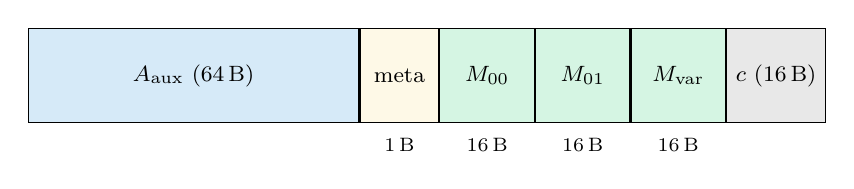
\begin{tikzpicture}[
    box/.style={draw, minimum height=1.2cm, text centered, font=\footnotesize},
    label/.style={font=\scriptsize, text centered}
]
\node[box, fill=fieldblue, minimum width=4.2cm] (eaux) at (0,0) {$A_{\mathrm{aux}}$ (64\,B)};
\node[box, fill=metayellow, minimum width=1.0cm, right=0pt of eaux] (meta) {meta};
\node[box, fill=matrixgreen, minimum width=1.2cm, right=0pt of meta] (m00) {$M_{00}$};
\node[box, fill=matrixgreen, minimum width=1.2cm, right=0pt of m00] (m01) {$M_{01}$};
\node[box, fill=matrixgreen, minimum width=1.2cm, right=0pt of m01] (mvar) {$M_{\mathrm{var}}$};
\node[box, fill=challgray, minimum width=1.2cm, right=0pt of mvar] (ch) {$c$ (16\,B)};

\node[label, below=2pt of meta] {1\,B};
\node[label, below=2pt of m00] {16\,B};
\node[label, below=2pt of m01] {16\,B};
\node[label, below=2pt of mvar] {16\,B};
\end{tikzpicture}
\end{center}

\noindent
Fields not labeled are fixed-size: $A_{\mathrm{aux}}$ is always 64~bytes
and $\mathsf{chl}$ is always 16~bytes at Level~I. The metadata byte
encodes $r_{\mathrm{rsp}}$, $h$, and $n_{\mathrm{bt}}$ as described
in~\S\ref{sec:packing}. No challenge hints, no auxiliary hints, no
separate $n_{\mathrm{bt}}$ or $r_{\mathrm{rsp}}$ bytes.

\subsection{Sizes across security levels}
\label{sec:sizes}

\begin{center}
\begin{tabular}{l r r r}
\toprule
\textbf{Format} & \textbf{Level I} & \textbf{Level III} & \textbf{Level V} \\
\midrule
Standard & 148\,B & 224\,B & 292\,B \\
Compressed & 129\,B & 196\,B & 257\,B \\
Savings & 19\,B (13\%) & 28\,B (12\%) & 35\,B (12\%) \\
\bottomrule
\end{tabular}
\end{center}

\noindent
% source: Fp2 bytes 64/96/128, entry bytes 16/25/32, challenge bytes
% 16/24/32 (spec Appendix B and the crate's constants at v0.4.31):
% compressed = Fp2 + 1 + 3 x entry + challenge = 129 / 196 / 257;
% standard = 4 + Fp2 + 4 x entry + challenge = 148 / 224 / 292.
The savings grow in bytes at higher levels because the dropped entry
grows with $\lambda$. They shrink as a fraction because the
$A_{\mathrm{aux}}$ field, which these techniques do not touch, is a
larger part of the total.

\subsection{Security considerations}

The compressed format is a deterministic, invertible transformation of the
standard format. Given a standard signature, compression produces a unique
compressed signature, and decompression recovers the original matrix
$\mathbf{M}_{\mathrm{chl}}$ exactly. On the KAT vectors the decompressed
signature is byte-identical to the original on 100 of 100 at each level.
% source: kat_compressed.rs on branch fix/compressed-nbt-round2 (v0.4.31 with
% the format of Section 5), nist-v2 vectors, run 2026-10-23: measurements/round2/logs/kat_compressed_fix.log.
The verifier detects a failed decompression because the recovered matrix
must produce a valid Kani $(2,2)$-isogeny. An incorrect
$\det(\mathbf{M})$ or a corrupted matrix entry makes the isogeny
construction fail or the final hash check reject. Aardal et
al.~\cite{sqisign-security} prove the security of SQIsign v2.0 for the
standard signature format. Decompression is a preprocessing step that
either reproduces the standard-format matrix exactly or causes
verification to reject, so the security reduction applies to the
compressed format without modification.

%% ============================================================
\section{Pairing selection and negative results}
\label{sec:negative}
%% ============================================================

We analyze the choice of pairing (\S\ref{sec:tate-analysis}), report
the distributions behind the metadata byte (\S\ref{sec:hint-neg}), and
document two approaches to further compression that turn out to need
changes to the signer (\S\ref{sec:param-neg}).

\subsection{Tate pairing: degeneracy and the order of its values}
\label{sec:tate-analysis}

The Tate pairing costs one cubical ladder where the Weil pairing costs
two, and the specification uses it for its own change-of-basis
computation (Algorithm~2.5). This section derives what one Tate ladder per curve can recover, and measures it.

\paragraph{The transmitted basis is divisible.}
The verifier does not hold a basis of $E_{\mathrm{chl}}[2^N]$ chosen at
random; it holds $A = [2^{F - N}] P^{\mathrm{det}}$ and $B = [2^{F - N}]
Q^{\mathrm{det}}$ for points of order $2^F$ (\S\ref{sec:setting}). The
reduced Tate pairing of order $n$ is a map $t_n : E[n] \times
E(\mathbb{F}_{p^2}) / n E(\mathbb{F}_{p^2}) \to \mu_n$ (Section~2.2.5.1 of
the specification). For the curves at hand $E(\mathbb{F}_{p^2}) \cong
(\mathbb{Z}/(p + 1)\mathbb{Z})^2$, whose 2-primary part is
$(\mathbb{Z}/2^F\mathbb{Z})^2$, so the 2-primary part of the quotient by
$2^N E(\mathbb{F}_{p^2})$ is $(\mathbb{Z}/2^N\mathbb{Z})^2$. In it the
class of $B = [2^{F - N}] Q^{\mathrm{det}}$ has order $2^{N - (F - N)} =
2^{2N - F}$ when $2N > F$, and is trivial otherwise. Hence
\[
  t_{2^N}(A, B) \in \mu_{2^{2N - F}},
  \qquad\text{and likewise } t_{2^N}(B, A).
\]
At level~I, $F = 248$ and $N = 128 - n_{\mathrm{bt}}$, so the value has
order at most $2^8$ against the $g = 126 - n_{\mathrm{bt}}$ bits the
recovery needs. The final exponentiation $(p^2 - 1) / 2^N$ has 2-adic
valuation $F - N + 1$; the loss is in the argument, not in the exponent.
% source: F = 248 and e_rsp = 126 from the notation table; 2 x 128 - 248 = 8.

\paragraph{Lengthening the ladder does not help.}
For $T$ of order $2^N$ and $m \geq N$, the function $f_{2^m, T}$ with
divisor $2^m (T) - 2^m (0_E)$ is $f_{2^N, T}^{2^{m - N}}$, so
$t_{2^m}(T, U) = f_{2^N, T}(U)^{2^{m - N} (p^2 - 1) / 2^m} = t_{2^N}(T, U)$.
A ladder of $2^m$ steps on the scaled points computes the same value for
every $m \geq N$. On the KAT vectors the values, their orders and the
bits they recover are identical for every $m$ from $N$ to $F$.
% source: paper_pairing_audit.rs, task2_tate_sweep, variant a.

\paragraph{Full-order points.}
The verifier also holds the points of order $2^F$ from which $(A, B)$ is
scaled, and can scale them to any order $2^m$ with $N \leq m \leq F$:
$A_m = [2^{F - m}] P^{\mathrm{det}}$, $B_m = [2^{F - m}] Q^{\mathrm{det}}$,
and likewise $(C_m, D_m)$ on $E_{\mathrm{aux}}$. The same argument gives
$t_{2^m}(A_m, B_m) \in \mu_{2^{2m - F}}$. Measured on the 300 KAT vectors
for every $m$ from $N$ to $F$, in both argument orders and on both
curves, the order is exactly $2^{\max(2m - F, 0)}$.
% source: paper_pairing_audit.rs, task2_tate_sweep, variant c, orders
% column: 2^(2m-F) on 100/100 per level at every m.

% for the co-author's review: the alternating claim below is the
% specification's sentence on page 15 (Section 2.2.5.1), quoted verbatim;
% the identity t^2 = e^((p^2-1)/n) that follows it is what the proposition
% and the measured threshold rest on.
\paragraph{The reduced Tate pairing is alternating here.}
On a maximal supersingular curve the reduced Tate pairing of order $n$ is alternating whenever $n$ divides
$p + 1$. Section~2.2.5.1 of the specification states: ``When
$E/\mathbb{F}_{p^2}$ is a maximal supersingular curve, and $n \mid p + 1$,
then the reduced Tate-Lichtenbaum pairing is alternate.'' So $t_n(T, T) = 1$ and $t_n(U, T) = t_n(T, U)^{-1}$, and
Step~1 of the proof of Theorem~\ref{thm:main} reads off
$\det \mathbf{M}$ from it exactly as from the Weil pairing. Moreover the
Weil pairing is the ratio $t_n(T, U) / t_n(U, T)$ of the two Miller
values before the final exponentiation (Section~8.3), so after it
\begin{equation}
\label{eq:tate-weil}
  t_n(T, U)^2 \;=\; e_n(T, U)^{(p^2 - 1)/n},
  \qquad
  \frac{p^2 - 1}{2^m} = 2^{F - m + 1} \cdot w,
  \quad w = c \,(c \, 2^{F - 1} - 1) \text{ odd}.
\end{equation}
This is where the cofactor $c$ enters, and only there: it also multiplies
the hint points when the deterministic basis is built (Algorithm~2.1,
lines 13 and 14), but both uses leave the odd exponent $w$, which is a
unit modulo $2^g$ and common to the two curves.

\begin{proposition}[recovery from one Tate ladder per curve]
\label{prop:tate}
Let $N \leq m \leq F$, let $\tau = t_{2^m}(A_m, B_m)$ and $\tau' =
t_{2^m}(C_m, D_m)$, and let $y_m = \log_\tau(\tau'^{-1})$ in the group
generated by $\tau$, which has order $2^{2m - F}$. Then
\[
  \det \mathbf{M} \;\equiv\; 2^{r_{\mathrm{rsp}}} \, y_m
  \pmod{2^{\min(g,\; 2m - F - 1 + r_{\mathrm{rsp}})}}.
\]
\end{proposition}

\begin{proof}
Let $\varepsilon = e_{2^F}(R, S)$ and $\varepsilon' = e_{2^F}(R', S')$ for
the full-order deterministic bases of the two curves, both of order
$2^F$, and $\lambda = \log_\varepsilon(\varepsilon'^{-1})$. By (W4) and
(W1), $\omega = \varepsilon^{2^{F - N}}$, $\eta = \varepsilon'^{2^{F - N +
r_{\mathrm{rsp}}}}$ and $e_{2^m}(A_m, B_m) = \varepsilon^{2^{F - m}}$, so
by~\eqref{eq:tate-weil} $\tau^2 = \varepsilon^{2^{2F - 2m + 1} w}$ and
$\tau'^2 = \varepsilon'^{2^{2F - 2m + 1} w}$. Squaring $\tau'^{-1} =
\tau^{y_m}$ and comparing exponents of $\varepsilon$ gives $\lambda
\equiv y_m \pmod{2^{2m - F - 1}}$. Step~4 of Theorem~\ref{thm:main} in
terms of $\varepsilon$ reads $\varepsilon^{2^{F - N} (\det \mathbf{M} -
2^{r_{\mathrm{rsp}}} \lambda)} = \zeta$ with $\zeta$ of order $4$, hence
$\det \mathbf{M} \equiv 2^{r_{\mathrm{rsp}}} \lambda \pmod{2^g}$.
Combining the two congruences gives the claim.
\end{proof}

The bit lost in the squaring is the sign of the square root
in~\eqref{eq:tate-weil}. On the KAT vectors it is not lost: the
congruence holds modulo $2^{\min(g, 2m - F + r_{\mathrm{rsp}})}$ on 300 of
300, so the two curves' Tate values take the same sign. One Tate ladder
per curve therefore recovers $\det \mathbf{M}$ as soon as $2m - F \geq g
- r_{\mathrm{rsp}}$, that is for
\[
  m \;\geq\; \Bigl\lceil \tfrac{F + g - r_{\mathrm{rsp}}}{2} \Bigr\rceil,
\]
which for $n_{\mathrm{bt}} = r_{\mathrm{rsp}} = 0$ is $187$, $284$ and
$377$ at the three levels. 

\paragraph{Measurement.}
Table~\ref{tab:sweep} summarizes the sweep over every $m$ from $N$ to $F$
on the 300 KAT vectors. The per-vector rule $m \geq \lceil (F + g -
r_{\mathrm{rsp}})/2 \rceil$ holds with equality on 300 of 300, and the
comparison with $-\det \mathbf{M}$ fails on every vector at every $m$.
% source: paper_pairing_audit.rs, task2_tate_sweep, variant c, the
% per-n_bt summary and the per-vector rule check (printed as
% "smallest working m == ceil((F + d - r')/2) on 100/100 vectors").

\begin{table}[H]
\centering
\caption{One Tate ladder per curve on the deterministic bases scaled to
order $2^m$: vectors (of 100 per level) on which the logarithm recovers
$\det \mathbf{M}$ modulo $2^g$, by $m$. On the transmitted bases of order
$2^N$ the count is 0 at every $m$.}
\label{tab:sweep}
\small
\begin{tabular}{l l l l}
\toprule
\textbf{Level} & \textbf{order of the value} & \textbf{vectors recovered, by $m$} & \textbf{all 100 from} \\
\midrule
I ($F = 248$, $N \leq 128$) & $2^{2m - F}$ & 0 up to 183; 3, 7, 35 at 184, 185, 186 & $m = 187$ \\
III ($F = 376$, $N \leq 194$) & $2^{2m - F}$ & 0 up to 279; 2, 3, 10, 49 at 280 to 283 & $m = 284$ \\
V ($F = 500$, $N \leq 255$) & $2^{2m - F}$ & 0 up to 373; 2, 14, 67 at 374, 375, 376 & $m = 377$ \\
\bottomrule
\end{tabular}
\end{table}

\paragraph{Cost.}
At level~I on KAT entry~0, medians of 201 iterations on the machine of
\S\ref{sec:cost}: the two Weil ladders of the decompressor, of 128 and
127 steps, take 187.2~$\mu$s on $E_{\mathrm{chl}}$; one Tate ladder of
187 steps takes about 152~$\mu$s, and 224.3~$\mu$s with the 61
doublings that bring the full-order basis to order $2^{187}$. The fair
comparison is the whole pairing stage. The decompressor first doubles
the full-order bases 120 and 121 times (286.5~$\mu$s for both curves)
and then runs two Weil ladders per curve (375.5~$\mu$s for both):
689.5~$\mu$s. The single-ladder stage doubles 61 times per curve and
runs one ladder per curve: 453.1~$\mu$s, 34\% less, which is 4\% of a
compressed verification (Table~\ref{tab:breakdown}). At $m = F$ no
doublings are needed and the ladder takes 181.8~$\mu$s per curve.
% source: paper_pairing_audit.rs, timing_l1_kat0 with PAPER_TATE_MC=187
% PAPER_TATE_M=188: Weil 187.2; variant c per curve 224.3 (doublings
% alone 72.4); both curves 453.1; production doublings 286.5, production
% pairing stage 689.5, two Weil pairings 375.5; single ladders at m =
% 128 / 188 / 248: 104.6 / 143.2 / 181.8 us.

\subsection{The metadata byte: distributions and non-eliminability}
\label{sec:hint-neg}

Table~\ref{tab:meta} gives the observed distributions of the three
fields of the metadata byte over the 300 official KAT vectors.
Table~\ref{tab:hint-contingency} gives the counts of the hint against the
other two fields and against the parity of $M_{00}$ at level~I.
% source: n_bt and r_rsp histograms: paper_stats.rs (c) on the nist-v2
% vectors at v0.4.31, run_stats2.log, cross-checked by reading the bytes
% of the .rsp files; h histograms and the contingency counts:
% kat_compressed.rs on branch fix/compressed-nbt-round2, run 2026-10-23,
% measurements/round2/logs/kat_compressed_fix.log; chi-square of h with
% 1 d.o.f. = (a - 50)^2/50 + (b - 50)^2/50.

\begin{table}[H]
\centering
\caption{Values of the metadata fields over 100 KAT vectors per level:
counts of each value, smallest value first.}
\label{tab:meta}
\small
\begin{tabular}{l l l l}
\toprule
\textbf{Field} & \textbf{Level I} & \textbf{Level III} & \textbf{Level V} \\
\midrule
$n_{\mathrm{bt}}$ ($0, 1, \ldots$) & 77, 20, 1, 2 & 68, 25, 5, 1, 1 & 74, 17, 7, 2 \\
$r_{\mathrm{rsp}}$ ($0, 1, \ldots$) & 48, 24, 18, 4, 3, 0, 2, 1 & 39, 25, 18, 10, 6, 0, 1, 0, 1 & 47, 30, 14, 5, 2, 2 \\
$h$ ($0, 1$) & 52, 48 & 50, 50 & 52, 48 \\
chi-square of $h$, 1 d.o.f. & 0.16 & 0.00 & 0.16 \\
\bottomrule
\end{tabular}
\end{table}

\begin{table}[H]
\centering
\caption{Level I: the hint bit $h$ against $n_{\mathrm{bt}}$, against $r_{\mathrm{rsp}}$ and against the parity of $M_{00}$, counts over 100 vectors.}
\label{tab:hint-contingency}
\small
\begin{tabular}{l l l l}
\toprule
$h$ & $n_{\mathrm{bt}} = 0, 1, 2, 3$ & $r_{\mathrm{rsp}} = 0, \ldots, 7$ & $M_{00}$ even, odd \\
\midrule
0 & 39, 11, 0, 2 & 28, 9, 9, 1, 2, 0, 2, 1 & 16, 36 \\
1 & 38, 9, 1, 0 & 20, 15, 9, 3, 1, 0, 0, 0 & 12, 36 \\
\bottomrule
\end{tabular}
\end{table}

We considered three strategies for eliminating the hint bit $h$.

\emph{Signer retry.} The signer could reject signatures whose hint does
not match a fixed target, say $h = 0$, and sign again with fresh
randomness. With $\Pr[h = 0] = 1/2$ the expected number of attempts is 2, and 95\%
success needs 5. Level~I signing costs about 100~Mcycles in the
reference implementation (Table~2 of the specification), so this is a
slowdown of 2 to 5 times for one bit.
% source: sqisign-spec-r2 Table 2 (signing 101.6 Mcycles at NIST-I).

\emph{Algebraic elimination.} Proposition~\ref{prop:precision} says what the pairings determine:
$\det \mathbf{M}$ modulo $2^{N - 1}$ from the logarithm at order $2^N$.
The remaining bit is the top bit of $u$ in equation~\eqref{eq:det-full},
a property of the signer's basis of $E_{\mathrm{com}}$ that the verifier
never sees.

\emph{Deriving from other signature fields.} The contingency counts
above show no dependence of $h$ on $n_{\mathrm{bt}}$, $r_{\mathrm{rsp}}$
or the parity of $M_{00}$ beyond what uniform sampling produces.

\subsection{Inferring the metadata from the matrix}
\label{sec:param-neg}

Reducing from 129 to 128~bytes would require eliminating the metadata
byte. Corollary~\ref{cor:valuation} gives $r_{\mathrm{rsp}} = v_2(\det
\mathbf{M})$ once the matrix is known. But the matrix is known only after
the determinant has been recovered at a precision that itself depends on
$n_{\mathrm{bt}}$, and $n_{\mathrm{bt}}$ is not a function of the
matrix. We tested two readings of ``the matrix determines its
parameters'' on the KAT vectors.

\emph{Consistency.} For each vector we counted the pairs
$(n_{\mathrm{bt}}, r_{\mathrm{rsp}})$ with $0 \leq n_{\mathrm{bt}} \leq 3$
and $0 \leq r_{\mathrm{rsp}} \leq 15$ for which all four entries lie
below $2^{N(n_{\mathrm{bt}})}$, the bound of line~5 of Algorithm~4.9.
No vector at any level has exactly one consistent pair, and the reason is
structural. The bound depends on $n_{\mathrm{bt}}$ alone, so every value
of $r_{\mathrm{rsp}}$ is consistent whenever $n_{\mathrm{bt}}$ is, and
the count is always a multiple of 16. The weaker question, whether the
matrix determines $n_{\mathrm{bt}}$, has a partial answer. It does on
70, 61 and 67 of 100 vectors at the three levels, exactly those with
$n_{\mathrm{bt}} = 0$ and some entry with bit $e_{\mathrm{rsp}} + 1$ set.
% source: paper_stats.rs (e) on the nist-v2 vectors at v0.4.31: pairs
% per vector {16: 70, 32: 26, 48: 2, 64: 2} (L1), {16: 61, 32: 29, 48:
% 6, 64: 4} (L3), {16: 67, 32: 21, 48: 8, 64: 4} (L5).

\emph{A leading one.} A signer-side canonical form could place the
parameters in the top bits of an entry, for instance by forcing
$M_{00}$ to start with a $1$ followed by $r_{\mathrm{rsp}}$ and
$n_{\mathrm{bt}}$. The current signer does not do this. Bit $N - 1$ of
$M_{00}$ is set on 49, 52 and 58 of 100 vectors at the three levels, and
bit $N - 1$ of at least one entry on 92, 89 and 88. 
% source: paper_stats.rs (d) on the nist-v2 vectors at v0.4.31; the six
% readings tried: bit N-1, N-2, g-1, e_rsp+1, e_rsp-1, e_rsp-2 of M00,
% giving 49, 39, 52, 40, 55, 53 at level I.

Either route needs the signer to produce a canonical matrix, which the
v2.0 specification does not mandate; the round-3 specification does
mandate a canonical sign (\S\ref{sec:round3}), but not a canonical top
bit. The metadata byte stays.

%% ============================================================
\section{Implementation and performance}
\label{sec:impl}
%% ============================================================

\subsection{Implementation}

We implement a complete SQIsign v2.0 verifier in pure Rust. It has field
arithmetic ($\mathbb{F}_p$, $\mathbb{F}_{p^2}$), Montgomery curve
operations, the Weil pairing by the biextension cubical ladder,
deterministic basis generation, $(2,2)$-isogeny chains in theta
coordinates, and the verification flow with decompression.
The implementation covers all three NIST security levels and all three
signature formats (standard, expanded, compressed). The round-2 code measured in this paper is tag \texttt{v0.4.31} of the
crate~\cite{sqisign-rs}, the last round-2 release, with the format of \S\ref{sec:compression}; the round-3 format of
\S\ref{sec:round3} is in version 0.7.0.

Correctness is checked against the official NIST known-answer vectors of
the reference at tag \texttt{nist-v2}~\cite{the-sqisign-v2}, 100 per
level. Every standard signature verifies. Every signature converts to
the expanded format, which verifies after a byte round trip. Every signature compresses, decompresses to the byte-identical standard
signature and verifies compressed. The counts are 300, 300 and 300 of
300.
% source: standard and expanded: paper_stats.rs (g) at v0.4.31; compressed: kat_compressed.rs on branch fix/compressed-nbt-round2 (v0.4.31 with
% the format of Section 5), nist-v2 vectors, run 2026-10-23: measurements/round2/logs/kat_compressed_fix.log.
% source: paper_stats.rs (g) on the nist-v2 vectors at v0.4.31, run_stats2.log.

The verifier crate is \texttt{no\_std} with no heap allocation. All
intermediate buffers are stack-allocated with sizes fixed at compile time
by the parameter set. The crate contains no C code and no FFI calls.

\subsection{Verification cost and its components}
\label{sec:cost}

Table~\ref{tab:breakdown} is the cost of verification at level~I on KAT
entry~0 ($n_{\mathrm{bt}} = 0$, $r_{\mathrm{rsp}} = 1$). Each figure is
the median or the minimum of 200 timed iterations after 5 warm-ups with
\texttt{std::time::Instant}. Each component is timed in isolation on a
copy of the state the real flow feeds it. The machine is an Intel Xeon
at 2.80~GHz (Cascade Lake, a KVM guest with 32 virtual CPUs); the
compiler is \texttt{rustc} 1.99.0. The release build has fat LTO and
one codegen unit, supplied through the environment because the tag has
no release profile of its own, and \texttt{target-cpu=native} from the
tag's cargo configuration. Three runs agreed on every component median
to within 0.2\%.
% source: paper_timing.rs (paper_timing_level1_breakdown) in the
% v0.4.31 worktree, run_timing_primary1.log; runs 2 and 3 in
% run_timing_primary2.log and run_timing_primary3.log.

\begin{table}[H]
\centering
\caption{Level I verification cost in microseconds, KAT entry 0. The
count column says how many times the standard path (S) and the
compressed path (C) run the component.}
\label{tab:breakdown}
\small
\begin{tabular}{l c c r r r}
\toprule
\textbf{Component} & \textbf{S} & \textbf{C} & \textbf{median} & \textbf{S total} & \textbf{C total} \\
\midrule
decode signature & 1 & 1 & 0.2 & 0.2 & 0.2 \\
range check of $\mathbf{M}$, curve checks & 1 & 1 & 0.2 & 0.2 & 0.4 \\
challenge derivation $E_{\mathrm{pk}} \to E_{\mathrm{chl}}$ & 1 & 2 & 960.6 & 960.6 & 1921.3 \\
basis to hint on $E_{\mathrm{chl}}$ (hint check) & 1 & 2 & 25.6 & 25.6 & 51.2 \\
basis to hint on $E_{\mathrm{aux}}$ (hint check) & 1 & 2 & 21.9 & 21.9 & 43.7 \\
basis from hint, both curves & 1 & 1 & 28.3 & 28.3 & 28.3 \\
scaling the bases, both curves & 1 & 2 & 286.1 & 286.1 & 571.9 \\
Weil pairing on $E_{\mathrm{chl}}$, order $2^N$ & 0 & 1 & 188.4 & 0.0 & 188.4 \\
Weil pairing on $E_{\mathrm{aux}}$, order $2^{e' + 2}$ & 0 & 1 & 187.3 & 0.0 & 187.3 \\
inversions, point sums & 0 & 1 & 8.5 & 0.0 & 8.5 \\
discrete logarithm & 0 & 1 & 90.3 & 0.0 & 90.3 \\
entry recovery (inverse modulo $2^g$) & 0 & 1 & 0.4 & 0.0 & 0.4 \\
basis change, apply $\mathbf{M}$ & 1 & 1 & 533.6 & 533.6 & 533.6 \\
even part, $2^{r_{\mathrm{rsp}}}$-isogeny & 1 & 1 & 52.5 & 52.5 & 52.5 \\
$(2,2)$-isogeny chain & 1 & 1 & 2163.2 & 2163.2 & 2163.2 \\
final hash and compare & 1 & 1 & 57.0 & 57.0 & 57.0 \\
\midrule
sum of component medians & & & & 4129.3 & 5898.1 \\
full verification from bytes, median & & & & 4286.0 & 6005.7 \\
full verification from bytes, minimum & & & & 4102.3 & 5902.8 \\
\bottomrule
\end{tabular}
\end{table}

The component sums fall short of the full measurements by 3.7\% on the
standard path and 1.8\% on the compressed path, the cost of the glue
between components. The compressed path costs 1720~$\mu$s more than the
standard one at level~I, 40\%. At levels III and V the full medians are
11414 against 16629~$\mu$s and 23956 against 34258~$\mu$s, 46\% and
43\%.
% source: run_timing_primary1.log, level 3 and level 5 full medians.

The table says where that overhead is, and two costs follow from it.
The separate path, which the round-2 code measured here implements,
runs decompression as its own step that produces a standard signature
and hands it to the standard verifier. It therefore repeats the challenge derivation, the two basis generations
and the two basis scalings, 1294~$\mu$s of the 1769~$\mu$s of
decompression-only components. It costs 1720~$\mu$s over the 4286 of a
standard verification: 40\% at level~I, 46 and 43\% at levels III and V. The integrated path shares the challenge derivation and the basis work
with verification and adds only the two Weil pairings, the inversions
and point sums, the discrete logarithm and the entry recovery. From the
table that is $375.7 + 8.5 + 90.3 + 0.4 = 474.9$~$\mu$s, 11\% of a
standard verification. No extra basis scaling is needed, because the verifier
already scales both bases to the orders the pairings use. The round-3
implementation of \S\ref{sec:round3} is integrated and measures 13 to
18\%. The pairings alone are 376~$\mu$s, 6\% of the separate path's
compressed verification.
% source: the C column of the table: 960.6 + 51.2/2 + 43.7/2 + 571.9/2
% = 1293.8 duplicated; 188.4 + 187.3 + 8.5 + 90.3 + 0.4 = 474.9 unique.

Without \texttt{target-cpu=native} the full medians are 4394 and
6256~$\mu$s at level~I; with the tag's own default profile (no
cross-crate LTO) they are 4504 and 6229. The absolute figures are those
of this machine and build and are not comparable to figures on other
hardware.
% source: run_timing_portable2.log and run_timing_tagdefault2.log.

%% ============================================================
\section{Round 3}
\label{sec:round3}
%% ============================================================

The round-3 specification~\cite{sqisign-spec-r3} of 1 September 2026
changes the primes to $3 \cdot 2^{324} - 1$, $27 \cdot 2^{500} - 1$ and
$17 \cdot 2^{664} - 1$ (its Chapter~5), after the attack of
Wesolowski~\cite{wes26}. It also simplifies the response. The quaternion
response has odd norm (Algorithm~3.18), so there is no even part and no
$r_{\mathrm{rsp}}$. The challenge has length $\lambda$ and there is no
backtracking count. The response bound is $e_{\mathrm{rsp}} = \lceil
\log_2 p / 2 \rceil + \lambda / 4 + 1 = 196, 302, 400$ (Table~5). Both
deterministic bases are scaled to order $2^{e_{\mathrm{rsp}} + 2}$
(Algorithm~3.24, lines 9 and 10). The matrix has entries in
$[0, 2^{e_{\mathrm{rsp}} + 2})$ and is normalized to the lexicographically
smaller of $\mathbf{M}$ and $-\mathbf{M}$ (Algorithm~3.10, applied at
line~19 of Algorithm~3.23 and checked at line~4 of Algorithm~3.24); this
removes the sign freedom described in~\cite{aux-freedom}. The signature
is $(\mathsf{chl}, E_{\mathrm{aux}}, \mathbf{M}_{\mathrm{chl}},
\mathsf{hint}_{\mathrm{aux}}, \mathsf{hint}_{\mathrm{chl}})$. It is
encoded in $2 \cdot \texttt{FP\_ENCODED\_BYTES} + 4 \cdot
\texttt{RESPONSE\_BYTES} + \texttt{CHALLENGE\_BYTES} + 2$ bytes with
$\texttt{RESPONSE\_BYTES} = \lceil (e_{\mathrm{rsp}} + 2) / 8 \rceil =
25, 38, 51$ (Chapter~6, Table~11): 200, 306 and 406 bytes. The full
matrix is transmitted. The specification does not compress it, as De~Feo's
replies of July and October 2026 anticipated (\S\ref{sec:intro}).
% source: sqisign-spec-r3 Chapter 5, Table 5, Algorithms 3.10, 3.18,
% 3.23, 3.24, Chapter 6 Table 11.

Theorem~\ref{thm:main} applies with $n_{\mathrm{bt}} = r_{\mathrm{rsp}} =
0$: $N = e_{\mathrm{rsp}} + 2$, $g = e_{\mathrm{rsp}}$, both pairings
are taken at order $2^N$, the determinant is odd, and a pivot among
$M_{00}$ and $M_{01}$ always exists. Our round-3 format, in version 0.7 of the crate~\cite{sqisign-rs}, transmits three entries of
$\lceil e_{\mathrm{rsp}} / 8 \rceil$ bytes (the low $e_{\mathrm{rsp}}$
bits), one byte holding bit $e_{\mathrm{rsp}}$ of those three entries,
the challenge, and the two hints. That is
$2 \cdot \texttt{FP\_ENCODED\_BYTES} + 3 \lceil e_{\mathrm{rsp}} / 8 \rceil
+ \lambda / 8 + 3 = 176, 269, 353$ bytes. The fourth entry is recovered modulo $2^{e_{\mathrm{rsp}} + 1}$, so its
bit $e_{\mathrm{rsp}}$ is computed, not sent. Three bits ride along
because the verifier's chain consumes the points $P$ and $Q$ themselves,
not only the kernel they generate, and its acceptance depends on bit $e_{\mathrm{rsp}}$ of every entry.
Verification does not depend on bit $e_{\mathrm{rsp}} + 1$ of the
entries, for two reasons in the specification. Adding
$2^{e_{\mathrm{rsp}} + 1}$ to an entry adds a point of order 2 to $P$ or
$Q$, and the chain of Algorithm~3.20 uses the two points only through
their multiples: the kernel $\langle [4] P, [4] Q \rangle$
(Algorithm~3.19) and the 8-torsion points above it that the gluing step
consumes (Section~2.4.1 of the v2.0 specification), none of which a
2-torsion summand changes. The sign check of Algorithm~3.24, line~4,
reads that bit only on the first entry that is neither $0$ nor
$2^{e_{\mathrm{rsp}} + 1}$, and the signer's own normalization
(Algorithm~3.10) leaves it zero there. The decompressor therefore leaves
bit $e_{\mathrm{rsp}} + 1$ zero in every entry and runs the standard
verification, sign check included, on the result. The round-2 format
carries the dropped entry's top bit in its hint so that the round trip
reproduces the signer's bytes (\S\ref{sec:hint}); the round-3 format does
not need to. The two hint bytes are kept; recomputing them as
in \S\ref{sec:hints} would give 174, 267 and 351 bytes and is not done in
the crate.
% source: crates/verify/src/compressed.rs at sqisign-rs 0.7 (branch fix/compressed-nbt; module
% header; compressed_bytes()).

Table~\ref{tab:round3} is the measurement on the 300 round-3 KAT vectors
of the reference~\cite{the-sqisign-v3} at tag \texttt{nist-v3}. Every
vector compresses, verifies compressed, and decompresses to a signature
the standard verifier accepts. The decompressed matrix equals the
signer's in 14, 14 and 13 of 100 cases and differs only in bit
$e_{\mathrm{rsp}} + 1$ of some entry on the other 86, 86 and 87, all of
which verify.
% source: cargo test -p sqisign-kat --release --test kat_compressed --
% --nocapture at sqisign-rs 0.7 (branch fix/compressed-nbt) on 2026-10-23 (the test file
% crates/kat/tests/kat_compressed.rs); runs twice with identical output.

\begin{table}[H]
\centering
\caption{The round-3 format on the 300 round-3 KAT vectors. Pivot path:
vectors with $M_{00}$ even, where $M_{11}$ is transmitted instead of
$M_{10}$.}
\label{tab:round3}
\footnotesize
\begin{tabular}{l r r r r r r}
\toprule
\textbf{Level} & \textbf{Standard} & \textbf{Compressed} & \textbf{Saved} & \textbf{Verified} & \textbf{Pivot} & \textbf{Exact} \\
\midrule
I   & 200\,B & 176\,B & 24\,B (12.0\%) & 100/100 & 32/100 & 14/100 \\
III & 306\,B & 269\,B & 37\,B (12.1\%) & 100/100 & 22/100 & 14/100 \\
V   & 406\,B & 353\,B & 53\,B (13.1\%) & 100/100 & 37/100 & 13/100 \\
\bottomrule
\end{tabular}
\end{table}

The recovery costs two Weil pairings at order $2^{e_{\mathrm{rsp}} + 2}$
and one discrete logarithm on top of a verification. On the crate's
benchmark machine that is 2.2, 5.2 and 11.0 Mcycles, 18, 17 and 13\% of
a verification under a prepared key~\cite{sqisign-rs}.
% source: sqisign-rs README and BENCH session of 2026-09-25 (Intel Xeon
% 2.8 GHz, rdtsc): prepared-key verify 11.9 / 29.9 / 86.2 Mcycles,
% compressed 14.1 / 35.1 / 97.2.

%% ============================================================
\section{Conclusion}
\label{sec:conclusion}
%% ============================================================

We have proved, from the definitions of the SQIsign v2.0 specification,
that $\omega^{\det \mathbf{M}} \eta$ is a primitive fourth root of unity,
for $\omega$ and $\eta$ the Weil pairings of the transmitted challenge and
auxiliary bases. This gives $\det \mathbf{M}$ modulo $2^{e_{\mathrm{rsp}} - n_{\mathrm{bt}}
+ 1}$, one bit short of the width the matrix is carried at. With a
one-bit hint, an adaptive pivot, recomputed basis hints and a packed
metadata byte the level~I signature shrinks from 148 to 129 bytes,
checked on the 300 NIST KAT vectors. The reduced Tate pairing cannot replace the Weil pairing here:
on the transmitted basis its values have order at most $2^{2N - F}$, and
a symmetric pairing does not see the determinant. On the round-3
parameters the same recovery gives 176, 269 and 353 bytes against 200,
306 and 406.

\paragraph{Why the bytes matter.}
SQIsign's value is its combined size, 65-byte public keys and 148-byte
signatures at level~I in round 2 (Table~1 of the specification). A
LoRaWAN uplink at spreading factor 7 carries at most 242 bytes of
payload, so a 129-byte signature leaves 113 bytes for the message where
148 leaves 94. A DNS response above 512 bytes falls back to TCP and
costs a round trip, and every byte of signature in a DNSSEC answer
comes out of that budget. In a TLS~1.3 handshake with a three-signature
chain the saving is 57 bytes; in a transparency log or a ledger it is
19 bytes per entry, permanently.
% source: Table 1 of sqisign-spec-r2 (65 / 148); LoRaWAN regional
% parameters, maximum application payload at SF7 (242 bytes); RFC 1035
% Section 4.2.1 (512-byte UDP limit).

\paragraph{Future work.}
A pairing-free recovery along the lines of Pereira and
Barreto~\cite{pereira-barreto} would need the Pohlig-Hellman step on the
verifier's curves rather than on $E_0$; whether that can be done at
useful cost is open. Reaching 128 bytes needs a signer-side canonical
matrix (\S\ref{sec:param-neg}). The dimension-4 compact format of the
same crate, 108 bytes at the round-2 parameters and 142 at round 3, is
the subject of a separate report~\cite{sqisign-rs}.
% source: sqisign-rs paper-dim4/BENCH.md, sizes table (round 2 dim 4:
% 108 bytes; round 3 dim 4: 142 bytes).

%% ============================================================
%% References
%% ============================================================

\begin{thebibliography}{DKLPW20}

\bibitem[BMP23]{festa}
  A.~Basso, L.~Maino, and G.~Pope.
  {FESTA}: fast encryption from supersingular torsion attacks.
  In \emph{ASIACRYPT 2023}, Part~VII, LNCS 14444, pp.~98--126.
  Springer, 2023.

\bibitem[DLRW24]{sqisignhd}
  P.~Dartois, A.~Leroux, D.~Robert, and B.~Wesolowski.
  {SQIsignHD}: new dimensions in cryptography.
  In \emph{EUROCRYPT 2024}, Part~I, LNCS 14651, pp.~3--32.
  Springer, 2024.
  \url{https://eprint.iacr.org/2023/436}

\bibitem[SQI25a]{sqisign-spec-r2}
  M.~A.~Aardal, G.~Adj, D.~F.~Aranha, A.~Basso, \emph{et al.}
  {SQIsign}: algorithm specifications and supporting documentation,
  version~2.0.
  NIST PQC Round~2 submission, February 2025.
  \url{https://sqisign.org/spec/sqisign-20250205.pdf}

\bibitem[PB21]{pereira-barreto}
  G.~C.~C.~F.~Pereira and P.~S.~L.~M.~Barreto.
  Isogeny-based key compression without pairings.
  In \emph{PKC 2021}, LNCS 12710, pp.~131--154.
  Springer, 2021.

\bibitem[DKLPW20]{sqisign-original}
  L.~De~Feo, D.~Kohel, A.~Leroux, C.~Petit, and B.~Wesolowski.
  {SQISign}: compact post-quantum signatures from quaternions and
  isogenies.
  In \emph{ASIACRYPT 2020}, Part~I, LNCS 12491, pp.~64--93.
  Springer, 2020.
  \url{https://eprint.iacr.org/2020/1240}

\bibitem[NIST]{nist-pqc-sig}
  NIST.
  Post-quantum cryptography: additional digital signature schemes.
  \url{https://csrc.nist.gov/projects/pqc-dig-sig}

\bibitem[BDD+24]{sqisign2d-west}
  A.~Basso, P.~Dartois, L.~De~Feo, A.~Leroux, L.~Maino, G.~Pope,
  D.~Robert, and B.~Wesolowski.
  {SQIsign2D-West}: the fast, the small, and the safer.
  In \emph{ASIACRYPT 2024}, Part~III, LNCS 15486, pp.~339--370.
  Springer, 2024.
  \url{https://eprint.iacr.org/2024/760}

\bibitem[NO24]{qfesta}
  K.~Nakagawa and H.~Onuki.
  {QFESTA}: efficient algorithms and parameters for {FESTA} using
  quaternion algebras.
  In \emph{CRYPTO 2024}, Part~V, LNCS 14924, pp.~75--106.
  Springer, 2024.
  \url{https://eprint.iacr.org/2023/1468}

\bibitem[CJL+17]{costello-compression}
  C.~Costello, D.~Jao, P.~Longa, M.~Naehrig, J.~Renes, and D.~Urbanik.
  Efficient compression of {SIDH} public keys.
  In \emph{EUROCRYPT 2017}, Part~I, LNCS 10210, pp.~679--706.
  Springer, 2017.

\bibitem[ZSP+18]{zanon2018}
  G.~H.~M.~Zanon, M.~A.~Simplicio~Jr., G.~C.~C.~F.~Pereira,
  J.~Doliskani, and P.~S.~L.~M.~Barreto.
  Faster isogeny-based compressed key agreement.
  In \emph{PQCrypto 2018}, LNCS 10786, pp.~248--268.
  Springer, 2018.
  \url{https://eprint.iacr.org/2017/1143}

\bibitem[NR19]{naehrig-renes}
  M.~Naehrig and J.~Renes.
  Dual isogenies and their application to public-key compression for
  isogeny-based cryptography.
  In \emph{ASIACRYPT 2019}, Part~II, LNCS 11922, pp.~243--272.
  Springer, 2019.

\bibitem[SQI26]{sqisign-spec-r3}
  M.~A.~Aardal, G.~Adj, D.~F.~Aranha, A.~Basso, \emph{et al.}
  {SQIsign}: algorithm specifications and supporting documentation,
  version~3.0.
  NIST PQC Round~3 submission, September 1, 2026.
  \url{https://sqisign.org/spec/sqisign-20260901.pdf}

\bibitem[Ray26]{issue19}
  D.~Ray.
  Technical notes on signature compression techniques.
  Issue~19 of \texttt{SQISign/the-sqisign}, opened 8 July 2026, with
  replies by L.~De~Feo of 8 July and 7 October 2026.
  \url{https://github.com/SQISign/the-sqisign/issues/19}

\bibitem[SQI25c]{the-sqisign-v2}
  The {SQIsign} team.
  \texttt{the-sqisign}, reference implementation, tag \texttt{nist-v2},
  commit \texttt{91e9e46}, 6 February 2025.
  \url{https://github.com/SQISign/the-sqisign}

\bibitem[SQI26b]{the-sqisign-v3}
  The {SQIsign} team.
  \texttt{the-sqisign}, reference implementation, tag \texttt{nist-v3},
  commit \texttt{6d01770}, 1 September 2026.
  \url{https://github.com/SQISign/the-sqisign}

\bibitem[Ray26b]{sqisign-rs}
  D.~Ray.
  \texttt{sqisign-rs}: {SQIsign} in pure {Rust}.
  Version 0.7 (round 3); the round-2 line at tag \texttt{v0.4.31} with
  the format of this paper on branch \texttt{fix/compressed-nbt-round2}, 2026.
  \url{https://github.com/anchorageoss/sqisign-rs}

\bibitem[Ray26c]{aux-freedom}
  D.~Ray.
  Auxiliary isogeny freedom in {SQIsign}'s two-dimensional
  representation.
  Cryptology ePrint Archive, 2026/1305, 2026.
  \url{https://eprint.iacr.org/2026/1305}

\bibitem[Wes26]{wes26}
  B.~Wesolowski.
  The supersingular isogeny problem in time and memory $p^{1/3 + o(1)}$.
  Cryptology ePrint Archive, 2026/1486, 2026.
  \url{https://eprint.iacr.org/2026/1486}

\bibitem[SQI25b]{sqisign-spec-v201}
  M.~A.~Aardal, G.~Adj, D.~F.~Aranha, A.~Basso, \emph{et al.}
  {SQIsign}: algorithm specifications and supporting documentation,
  version~2.0.1.
  July 2025.
  \url{https://sqisign.org/spec/sqisign-20250707.pdf}

\bibitem[NO25]{sqisign2dpush}
  K.~Nakagawa and H.~Onuki.
  {SQIsign2DPush}: faster signature scheme using 2-dimensional
  isogenies.
  Cryptology ePrint Archive, 2025/897, 2025.
  \url{https://eprint.iacr.org/2025/897}

\bibitem[ZSP+19]{zanon2019}
  G.~H.~M.~Zanon, M.~A.~Simplicio~Jr., G.~C.~C.~F.~Pereira,
  J.~Doliskani, and P.~S.~L.~M.~Barreto.
  Faster key compression for isogeny-based cryptosystems.
  \emph{IEEE Trans.\ Comput.}\ \textbf{68}(5), pp.~688--701, 2019.

\bibitem[AAA+25]{aardal2024}
  M.~A.~Aardal, G.~Adj, A.~Alblooshi, D.~F.~Aranha,
  I.~A.~Canales-Mart\'{\i}nez, J.~Ch\'avez-Saab,
  D.~L.~Gazzoni~Filho, K.~Reijnders, and
  F.~Rodr\'{\i}guez-Henr\'{\i}quez.
  Optimized one-dimensional {SQIsign} verification on {Intel} and
  {Cortex-M4}.
  \emph{TCHES} 2025(1), pp.~497--522, 2025.
  \url{https://eprint.iacr.org/2024/1563}

\bibitem[CKMR24]{apressqi}
  M.~Corte-Real~Santos, J.~Komada~Eriksen, M.~Meyer, and K.~Reijnders.
  {Apr\`esSQI}: extra fast verification for {SQIsign} using
  extension-field signing.
  In \emph{EUROCRYPT 2024}, Part~I, LNCS 14651, pp.~63--93.
  Springer, 2024.

\bibitem[KLY26]{kim2026}
  W.~Kim, C.~Lee, and H.~Yoo.
  Compact quaternion algorithms for {SQIsign}.
  Cryptology ePrint Archive, 2026/1031, 2026.
  \url{https://eprint.iacr.org/2026/1031}

\bibitem[DJWY26]{sqisign-arm}
  L.~De~Feo, L.-J.~Jian, T.-Y.~Wang, and B.-Y.~Yang.
  {SQIsign} on {ARM}.
  Cryptology ePrint Archive, 2026/394, 2026.
  \url{https://eprint.iacr.org/2026/394}

\bibitem[Rob24]{robert-pairings}
  D.~Robert.
  Fast pairings via biextensions and cubical arithmetic.
  Cryptology ePrint Archive, 2024/517, 2024.
  \url{https://eprint.iacr.org/2024/517}

\bibitem[PRRS+25]{pope-pairings}
  G.~Pope, K.~Reijnders, D.~Robert, A.~Sferlazza, and B.~Smith.
  Simpler and faster pairings from the {Montgomery} ladder.
  \emph{IACR Communications in Cryptology}, Vol.~2, No.~2, 2025.
  \url{https://eprint.iacr.org/2025/672}

\bibitem[ABDPW25]{sqisign-security}
  M.~A.~Aardal, A.~Basso, L.~De~Feo, S.~Patranabis, and
  B.~Wesolowski.
  A complete security proof of {SQIsign}.
  Cryptology ePrint Archive, 2025/379, 2025.
  \url{https://eprint.iacr.org/2025/379}

\bibitem[Sil86]{silverman}
  J.~H.~Silverman.
  \emph{The Arithmetic of Elliptic Curves}.
  Graduate Texts in Mathematics, vol.~106.
  Springer, 1986.

\bibitem[DeF17]{defeo-survey}
  L.~De~Feo.
  Mathematics of isogeny based cryptography.
  arXiv:1711.04062, 2017.
  \url{https://arxiv.org/abs/1711.04062}

\bibitem[CH17]{costello-hisil}
  C.~Costello and H.~Hisil.
  A simple and compact algorithm for {SIDH} with arbitrary degree
  isogenies.
  In \emph{ASIACRYPT 2017}, Part~II, LNCS 10625, pp.~303--329.
  Springer, 2017.

\bibitem[FS87]{fiat-shamir}
  A.~Fiat and A.~Shamir.
  How to prove yourself: practical solutions to identification and
  signature problems.
  In \emph{CRYPTO 1986}, LNCS 263, pp.~186--194.
  Springer, 1987.

\bibitem[DLLW23]{sqisign-deuring}
  L.~De~Feo, A.~Leroux, P.~Longa, and B.~Wesolowski.
  New algorithms for the {Deuring} correspondence: towards practical
  and secure {SQIsign} signatures.
  In \emph{EUROCRYPT 2023}, Part~V, LNCS 14008, pp.~659--690.
  Springer, 2023.

\bibitem[Kan97]{kani}
  E.~Kani.
  The number of curves of genus two with elliptic differentials.
  \emph{J.~f\"ur die reine und angewandte Mathematik},
  \textbf{485}, pp.~93--122, 1997.

\end{thebibliography}

\end{document}